% -*- coding: utf-8; -*-

\chapter{Resultados}
\label{ch:result}

	Este capítulo apresenta os resultados desta dissertação para volumes de malhas regulares conhecidos na literatura e simulações de reservatório de petróleo, respectivamente nas Seções~\ref{sec:result.reg}~e~\ref{sec:result.irreg}. Esses resultados serão comparados com os obtidos através da aplicação do método de \textit{Kindlmann e Durkin}~\cite{gordon}. Portanto, para os volumes oriundos de simulações de petróleo, suas derivadas também serão calculadas de acordo com a Subseção~\ref{subsec:my.nonstruct}.
	
	É preciso lembrar, contudo, que existem diversas técnicas de visualização volumétrica. Então, a análise feita será sempre em cima da função de transferência obtida e como esta foi capaz, ou não, de realçar as fronteiras do volume. Portanto, juntamente com a visualização volumétrica serão exibidas uma fatia do volume e sua respectiva função de transferência.
	
	A fim de facilitar a análise dos volumes e suas respectivas funções de transferência geradas pelos dois métodos, utilizou-se uma só escala de cores para todos os volumes, exibida na figura abaixo. O acesso à textura da escala é feito por $ v $, de forma que o primeiro texel é dado por $ v = 0 $ e o último por $ v = 255 $.

\begin{figure}[h]
	\centering
	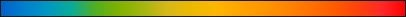
\includegraphics[width=0.9\textwidth]{images/r_colorscale}
	\caption{Escala de cores das funções de transferência.}
\end{figure}
	
\section{Malhas Regulares}
\label{sec:result.reg}

%%%%%%%%%%%%%%%%%%%%%%%%%%%%%%%%%% SPHERES %%%%%%%%%%%%%%%%%%%%%%%%%%%%%%%%%%%%%
\begin{figure}[h]
	\centering
	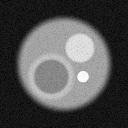
\includegraphics[width=0.25\textwidth]{images/r_3sphere_slice}
	\caption{Fatia do volume \quote{Test Spheres}.}
\end{figure}

	A figura acima exibe uma fatia de um volume ruidoso que consiste em $ 5 $ esferas com sobreposição no intervalo de suas fronteiras.

\begin{figure}[t]
	\centering
	\subfigure[Método de \textit{Kindlmann e Durkin}.]
	{
		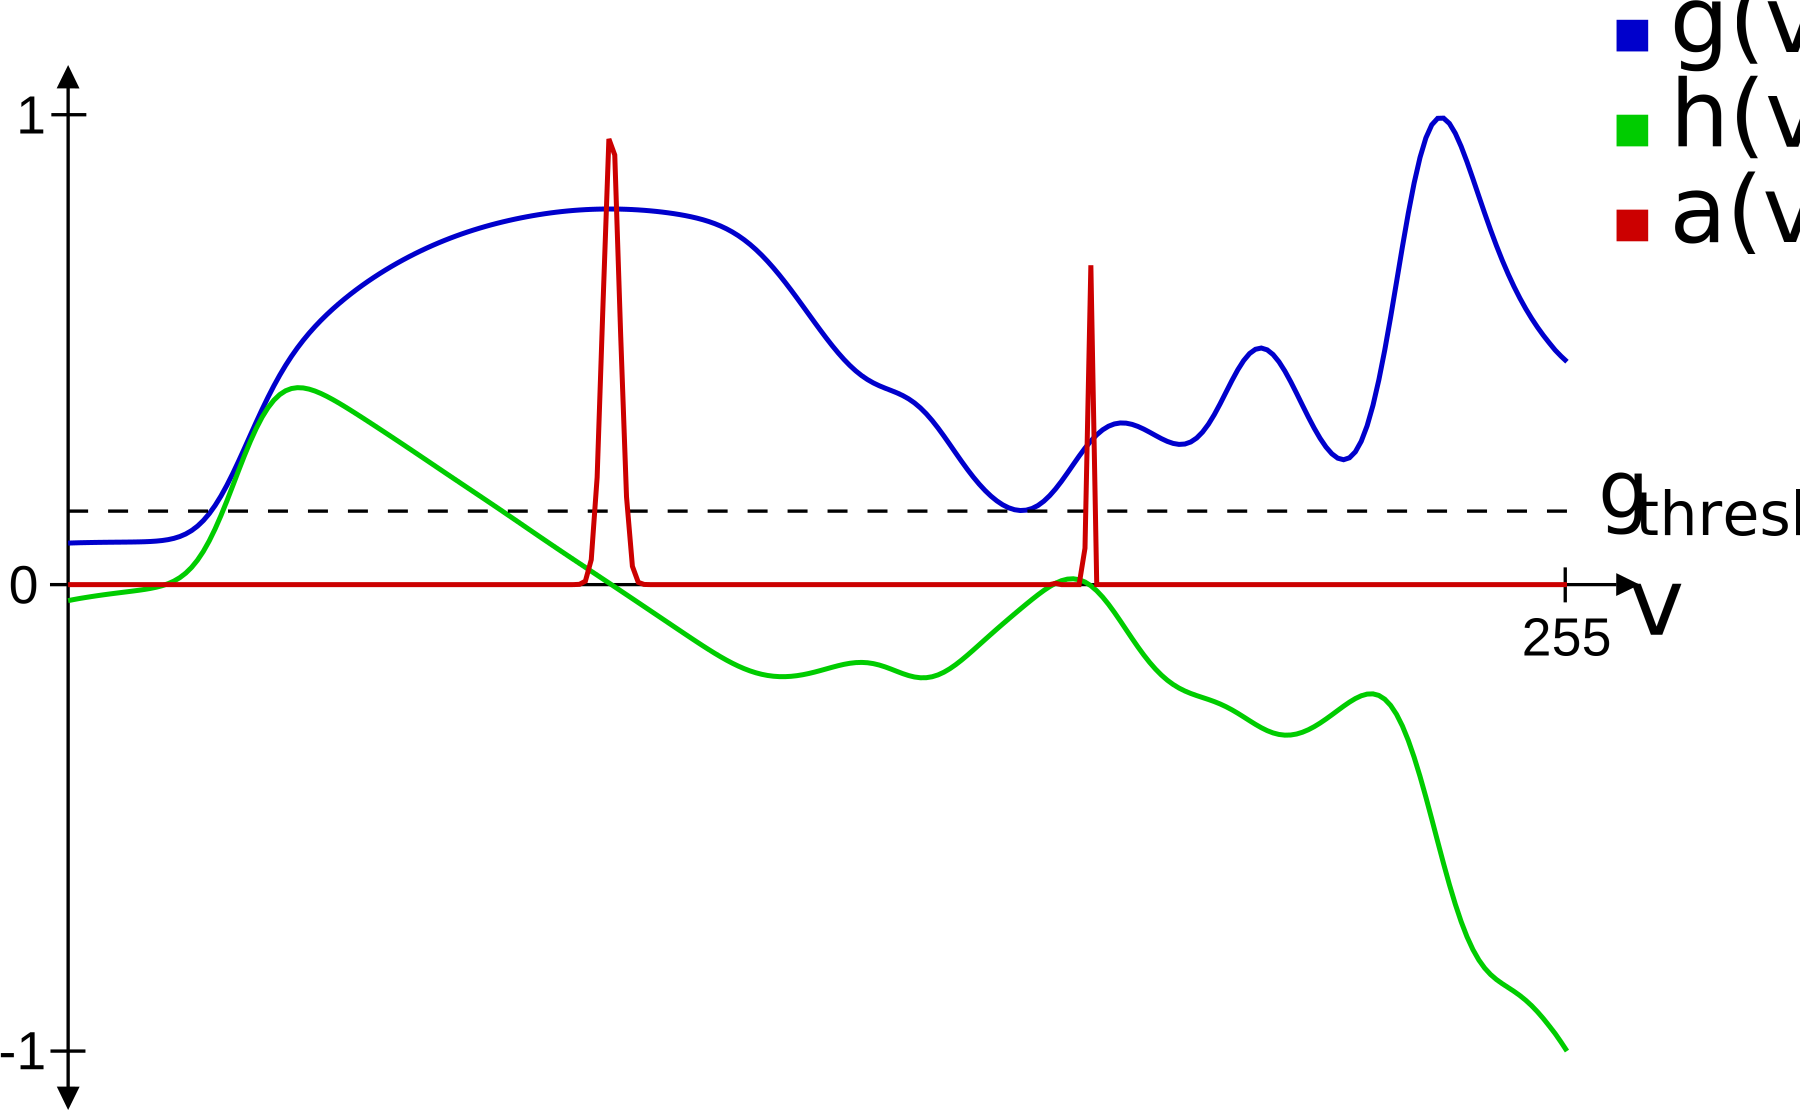
\includegraphics[width=0.35\textwidth]{images/r_g_3sphere}
		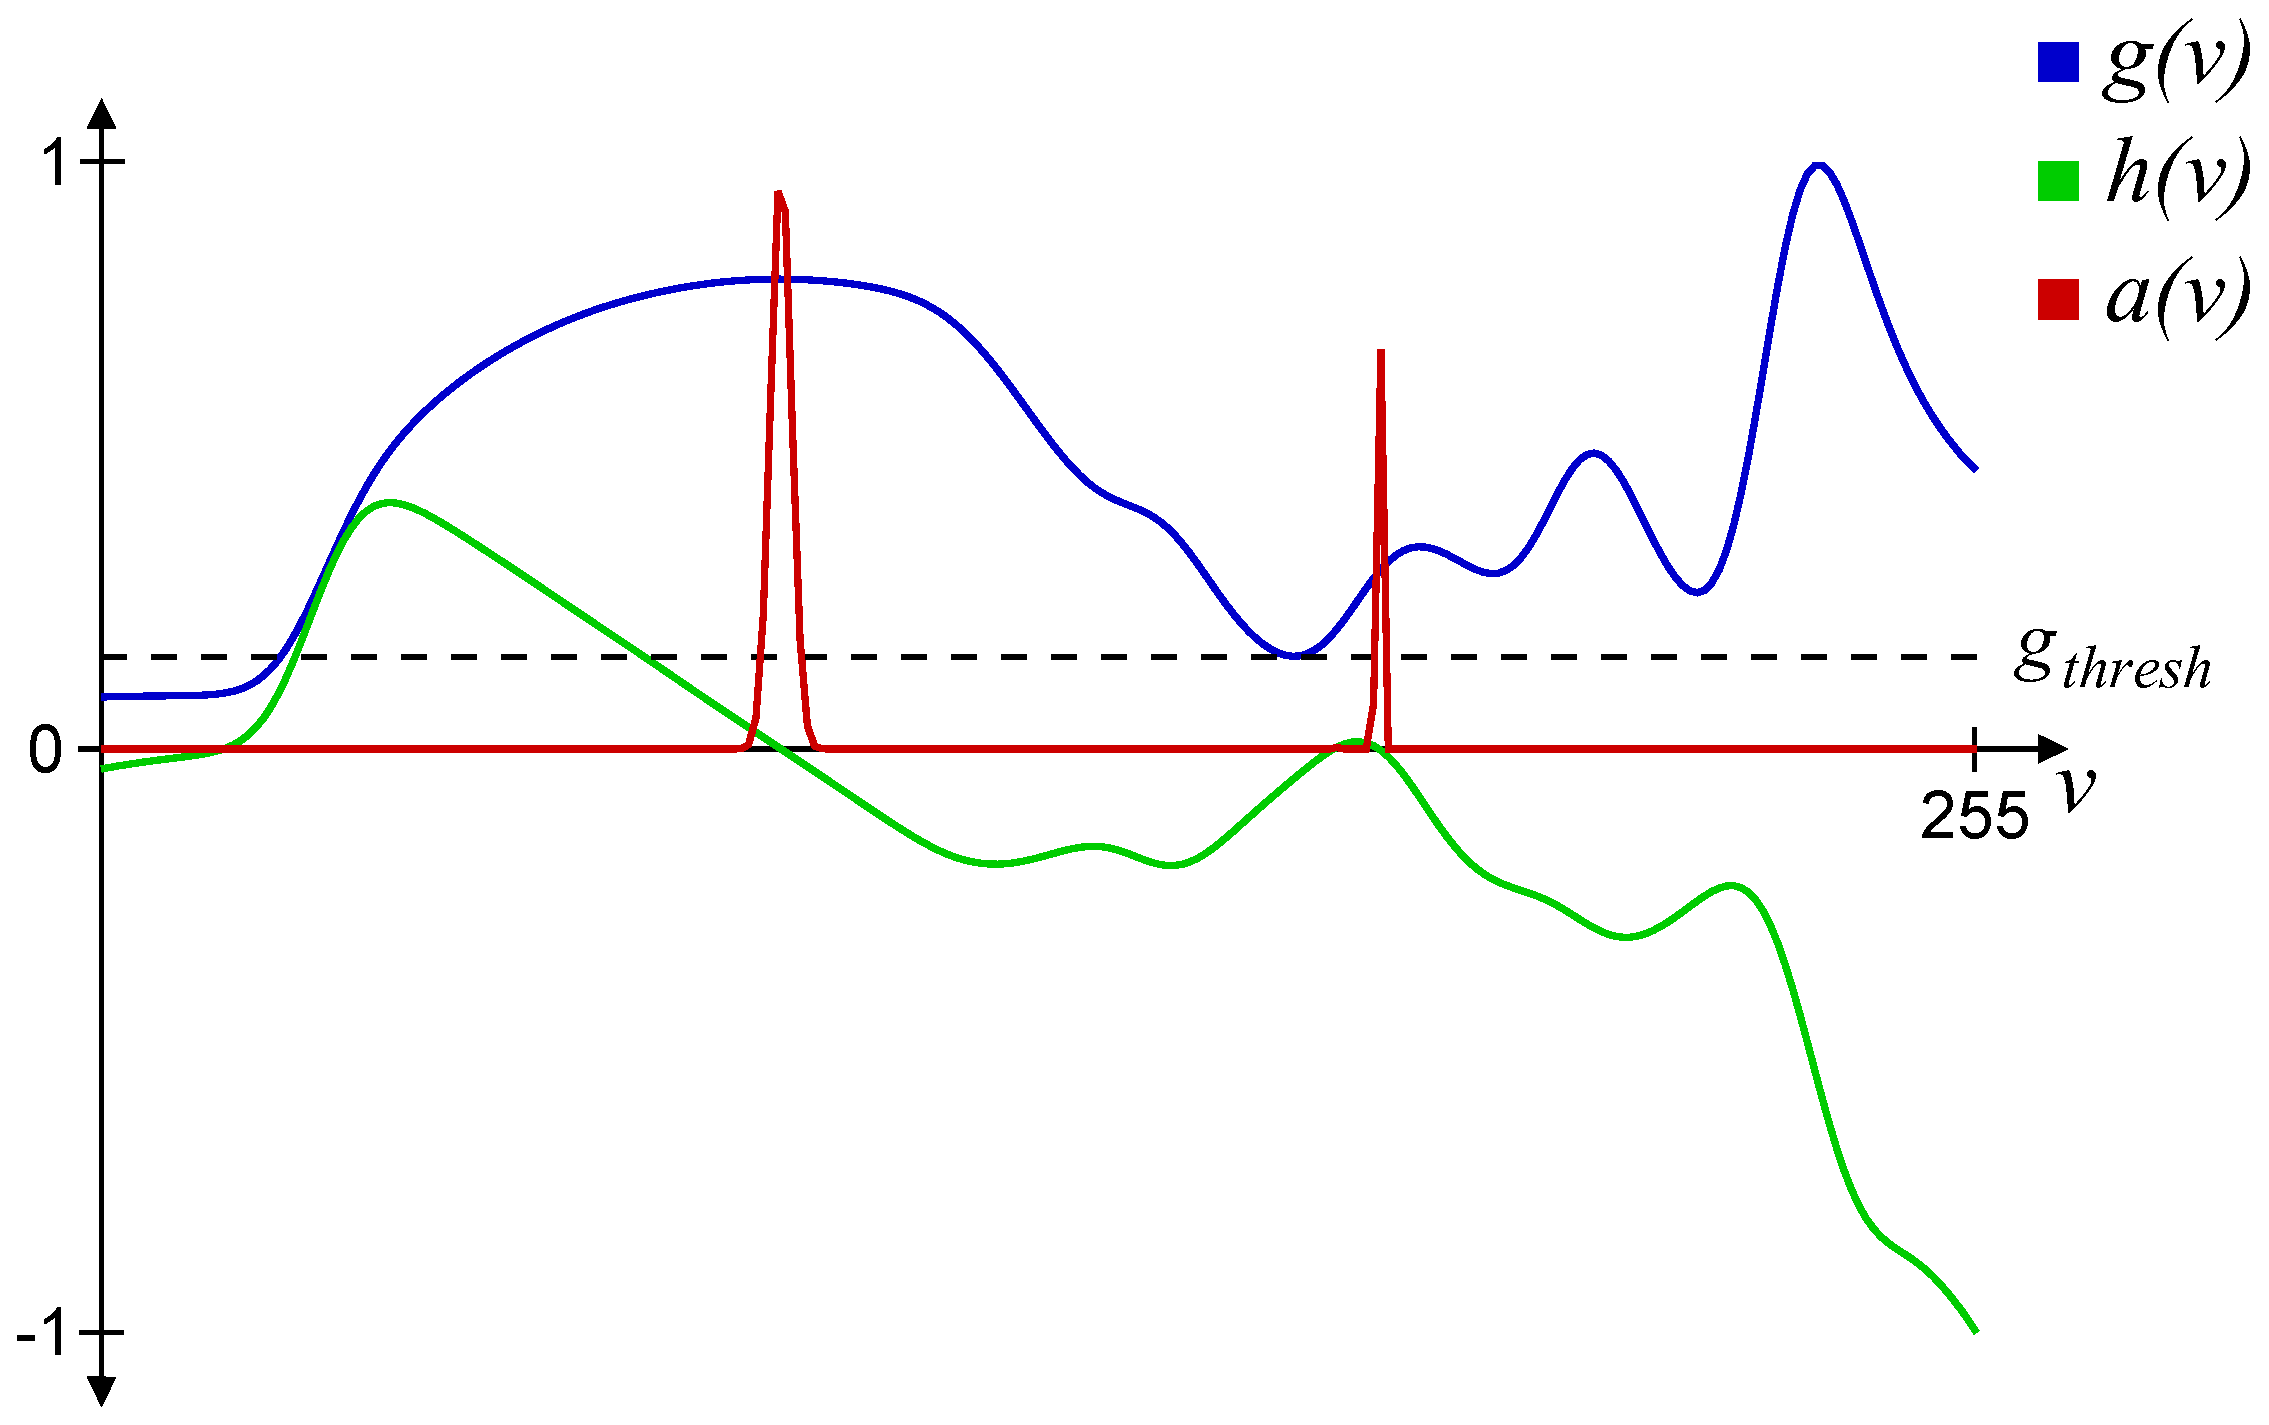
\includegraphics[width=0.65\textwidth]{images/r_g_3sphere_ft}
		\label{fig:r_3sphere_kd}
	}
	\subfigure[Método proposto.]
	{
		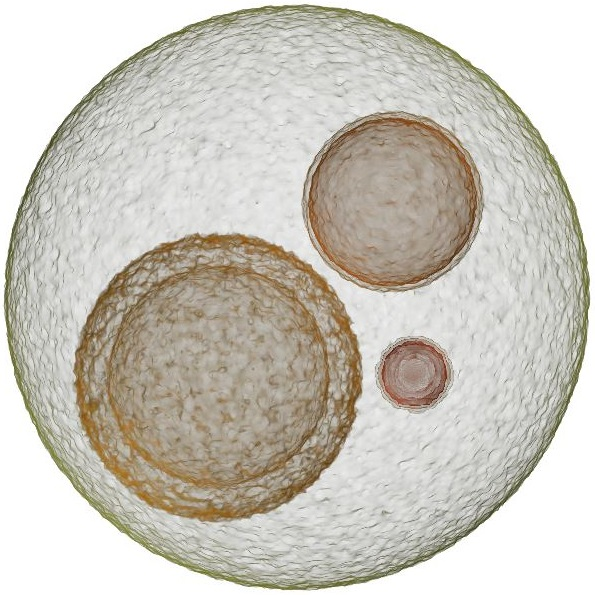
\includegraphics[width=0.35\textwidth]{images/r_m_3sphere}
		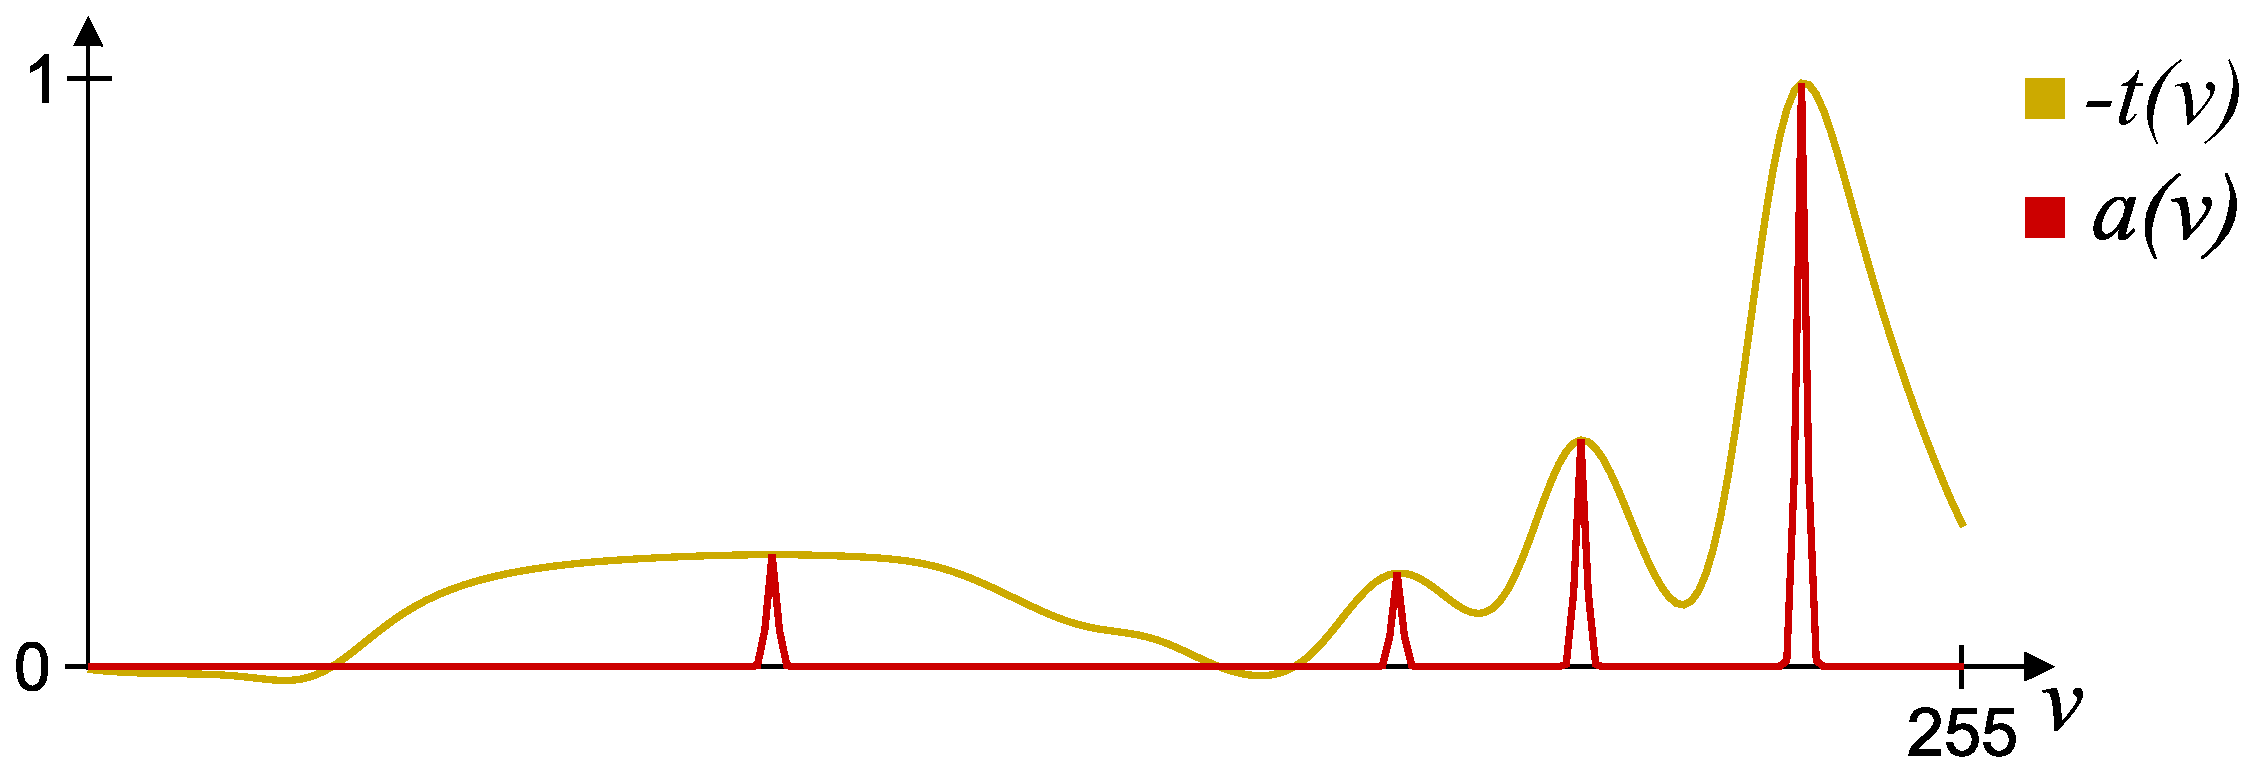
\includegraphics[width=0.65\textwidth]{images/r_m_3sphere_ft}			\label{fig:r_3sphere_mine}
	}
	\caption{Visualização e função de transferência do volume \quote{Test Spheres}.}
	\label{fig:r_3sphere}
\end{figure}

	A Figura~\ref{fig:r_3sphere} mostra que o método de \textit{Kindlmann e Durkin} apenas identifica $ 4 $ esferas. Conhecendo a escala de cores sabe-se que, na Figura~\ref{fig:r_3sphere}~\ref{fig:r_3sphere_kd}, o primeiro pico da FT corresponde à esfera mais externa, de cor verde, enquanto o segundo corresponde às outras, de tom alaranjado. No entanto, se apenas um pico realçou 3 fronteiras e há uma grande variação em sua opacidade conclui-se que a esfera menos opaca apenas foi capturada devido à sobreposição de intervalos. Na verdade, o método não a detectou. Jà o método proposto por esta dissertação identificou corretamente todas as esferas, como mostra a Figura~\ref{fig:r_3sphere}~\ref{fig:r_3sphere_mine}

%%%%%%%%%%%%%%%%%%%%%%%%%%%%%%%%%% NUCLEON %%%%%%%%%%%%%%%%%%%%%%%%%%%%%%%%%%%%%
\begin{figure}[h]
	\centering
	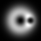
\includegraphics[width=0.25\textwidth]{images/g_nucleon_slice}
	\caption{Fatia do volume \quote{Nucleon}.}
	\label{fig:r_nucleon_slice}
\end{figure}

\begin{figure}[t]
	\centering
	\subfigure[Método de \textit{Kindlmann e Durkin}.]
	{
		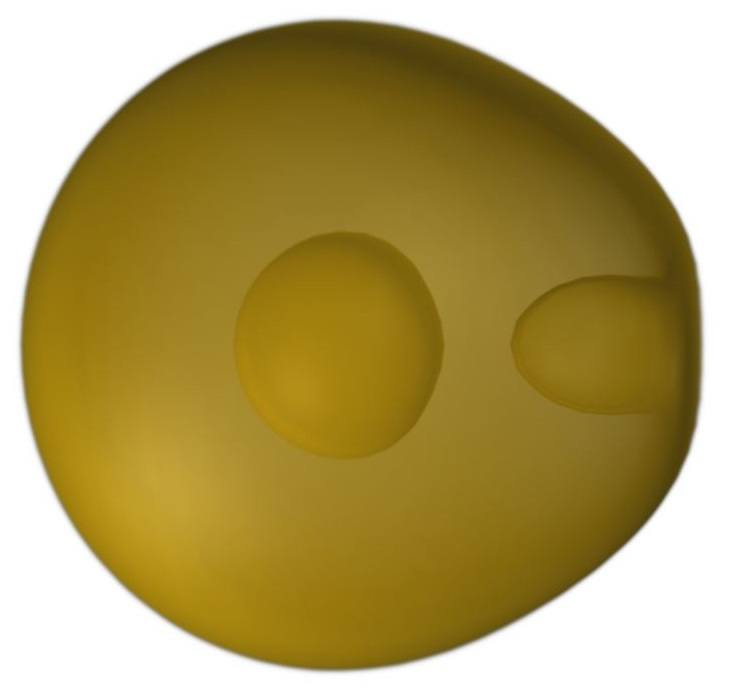
\includegraphics[width=0.35\textwidth]{images/g_nucleon}
		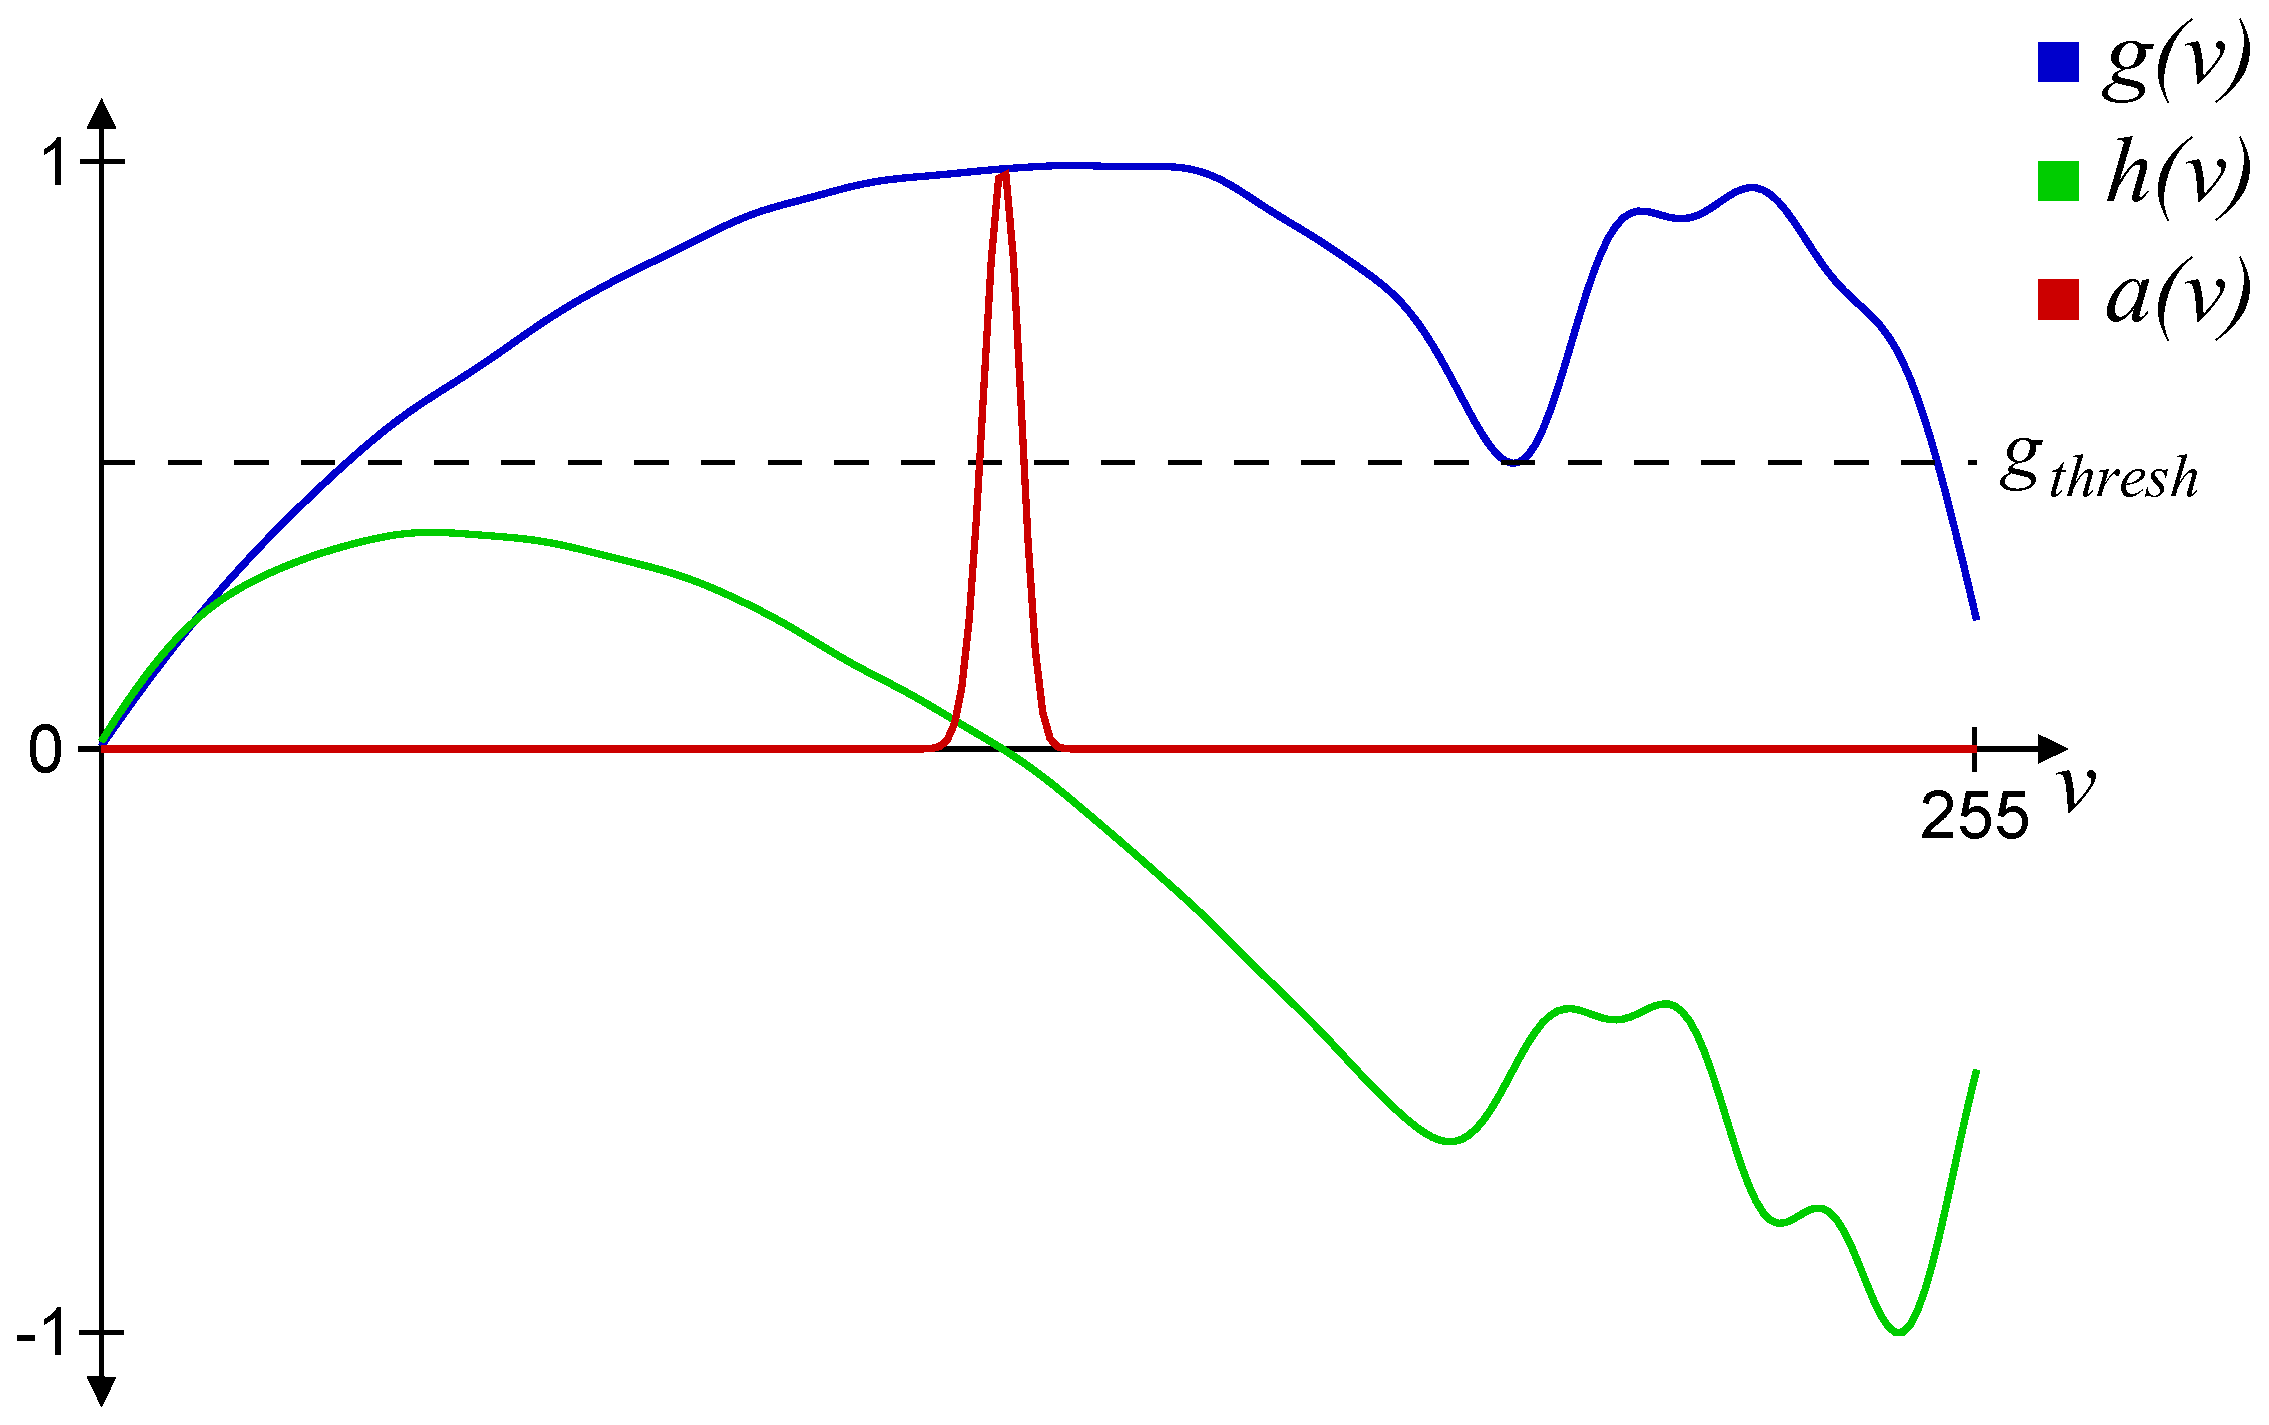
\includegraphics[width=0.65\textwidth]{images/r_g_nucleon_ft}
		\label{fig:r_nucleon_kd}
	}
	\subfigure[Método proposto.]
	{
		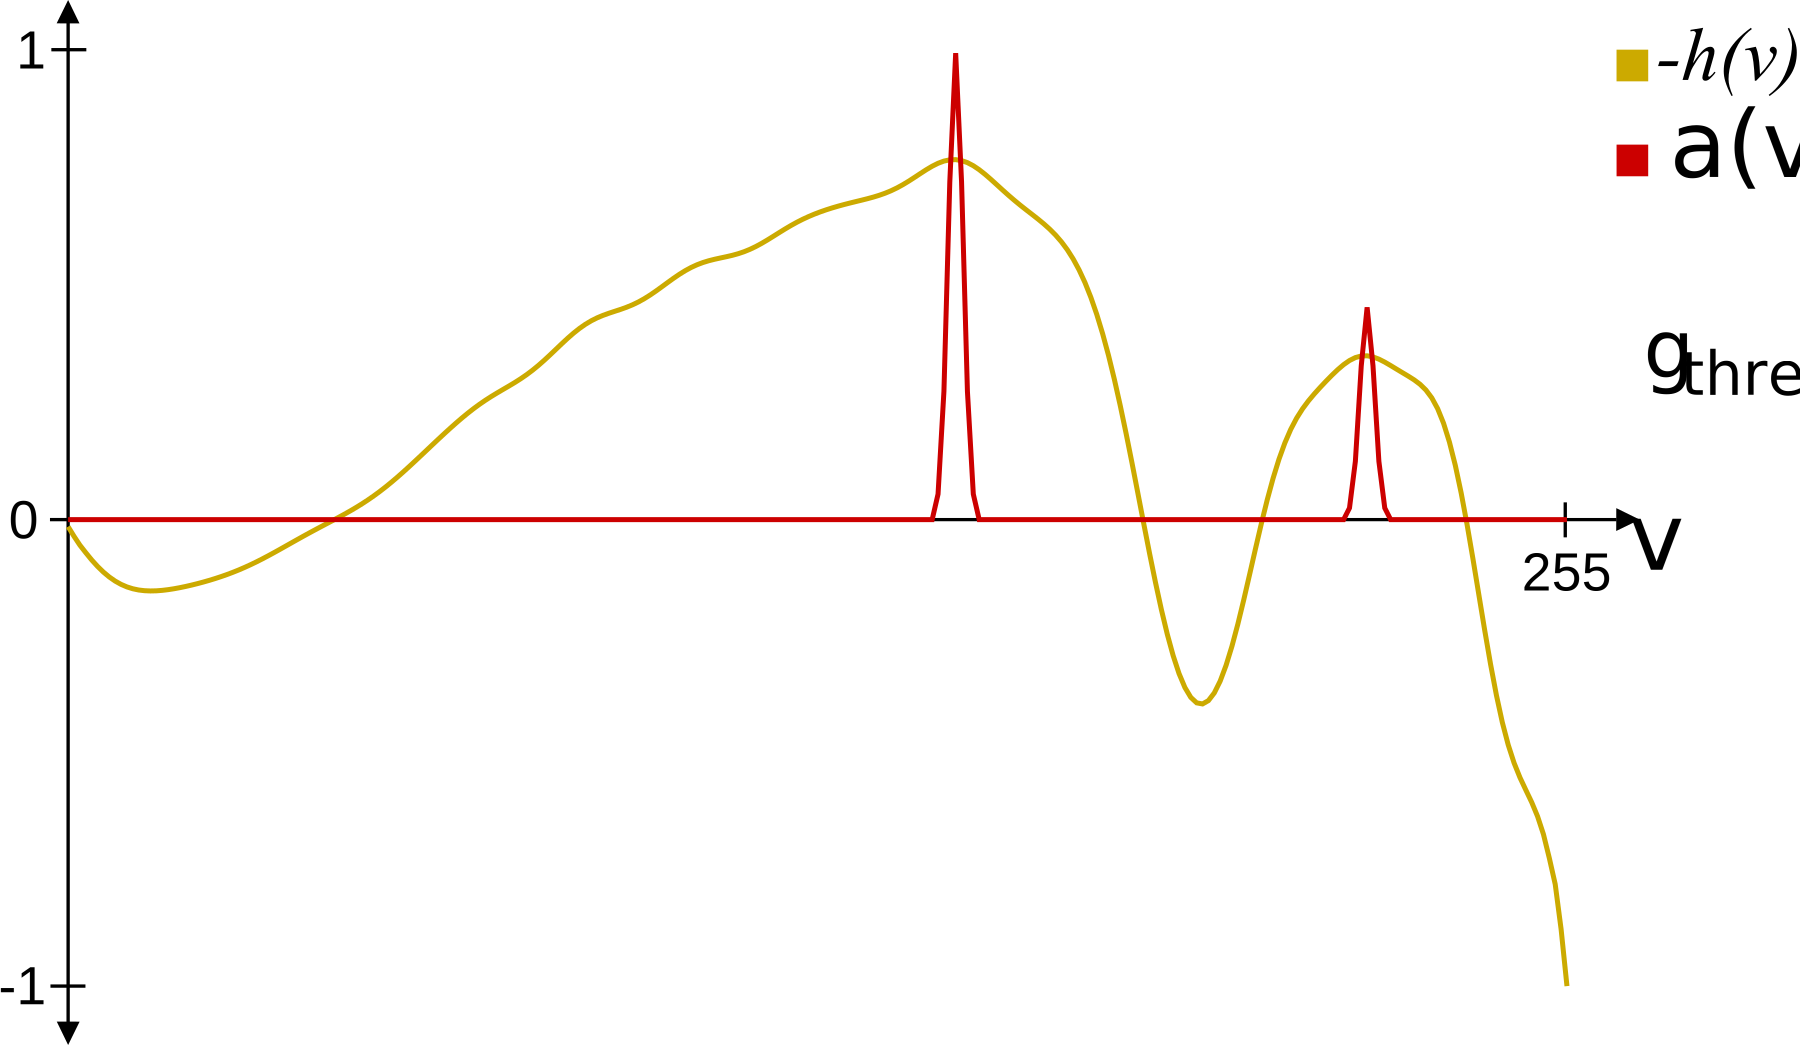
\includegraphics[width=0.35\textwidth]{images/r_m_nucleon}
		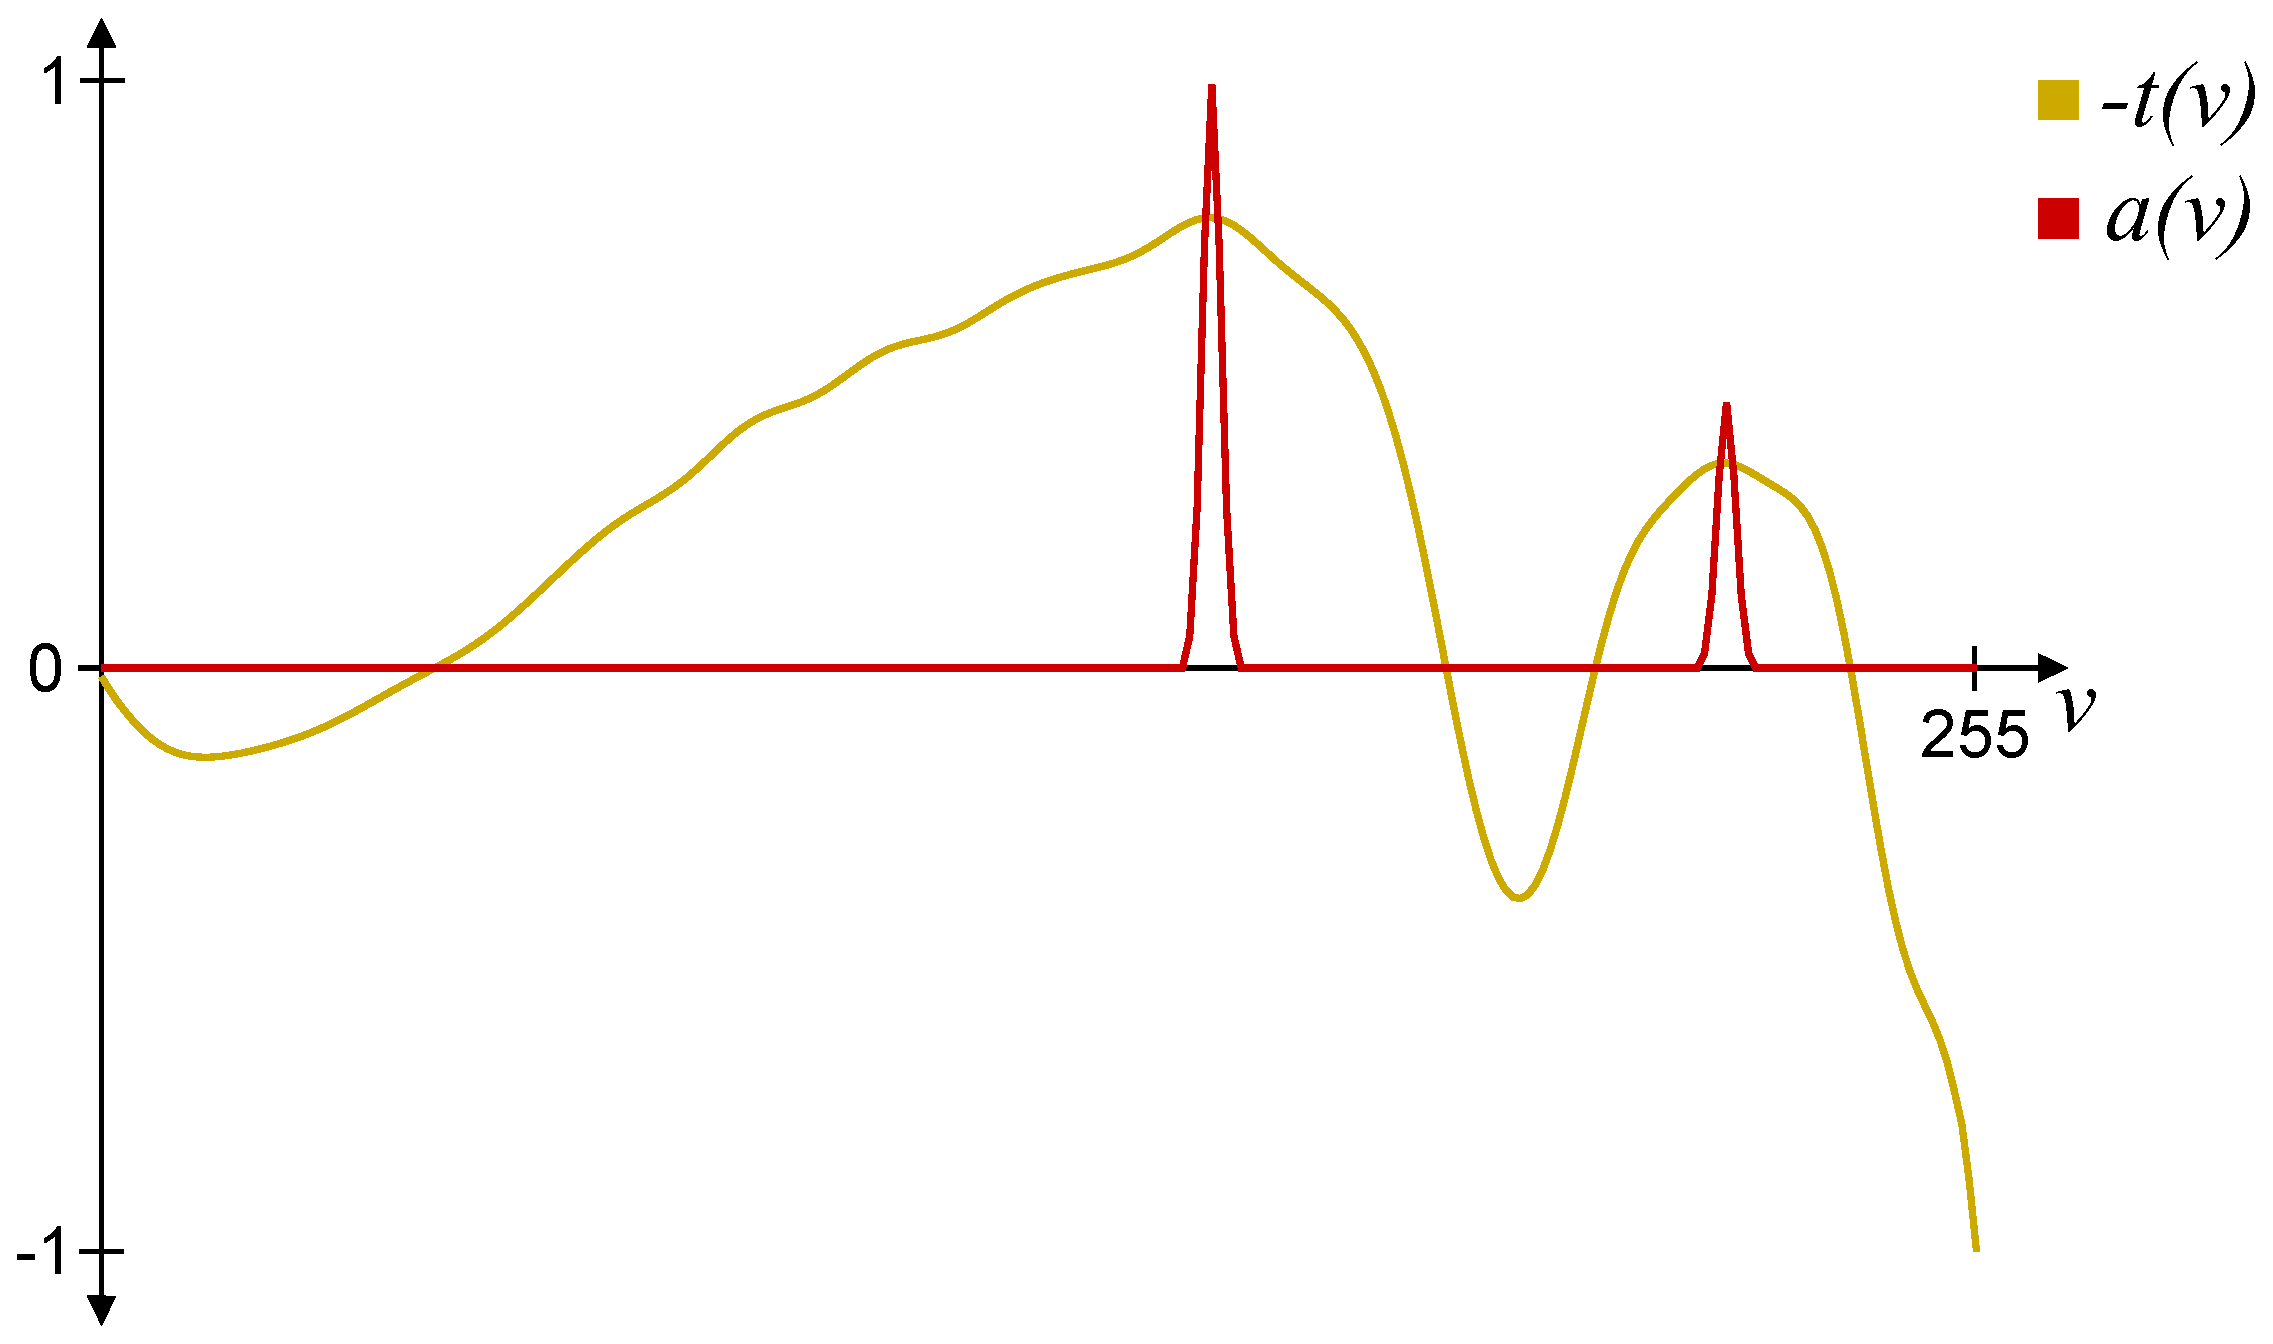
\includegraphics[width=0.65\textwidth]{images/r_m_nucleon_ft}			\label{fig:r_nucleon_mine}
	}
	\caption{Visualização e função de transferência do volume \quote{Nucleon}.}
	\label{fig:r_nucleon}
\end{figure}

A Figura~\ref{fig:r_nucleon} mostra mais um caso em que o método de \textit{Kindlmann e Durkin} não identifica todas as fronteiras existentes. Através da fatia do volume \quote{Nucleon}, exibida na Figura~\ref{fig:r_nucleon_slice}, vê-se que existem 2 fronteiras: cinza-preto e branco-preto. Porém, como ilustra a Figura~\ref{fig:r_nucleon}~\ref{fig:r_nucleon_kd}, apenas uma fronteira é realçada: a equivalente à transição cinza-preto na fatia do volume. Já o método proposto nesta dissertação identifica corretamente as duas fronteiras, como mostra a Figura~\ref{fig:r_nucleon}~\ref{fig:r_nucleon_mine}.
	
%%%%%%%%%%%%%%%%%%%%%%%%%%%%%%%%%% ENGINE %%%%%%%%%%%%%%%%%%%%%%%%%%%%%%%%%%%%%
\begin{figure}[h]
	\centering
	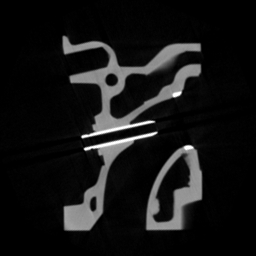
\includegraphics[width=0.3\textwidth]{images/r_engine_slice}
	\caption{Fatia do volume \quote{Engine}.}
	\label{fig:r_engine_slice}
\end{figure}

\begin{figure}[t]
	\centering
	\subfigure[Método de \textit{Kindlmann e Durkin}.]
	{
		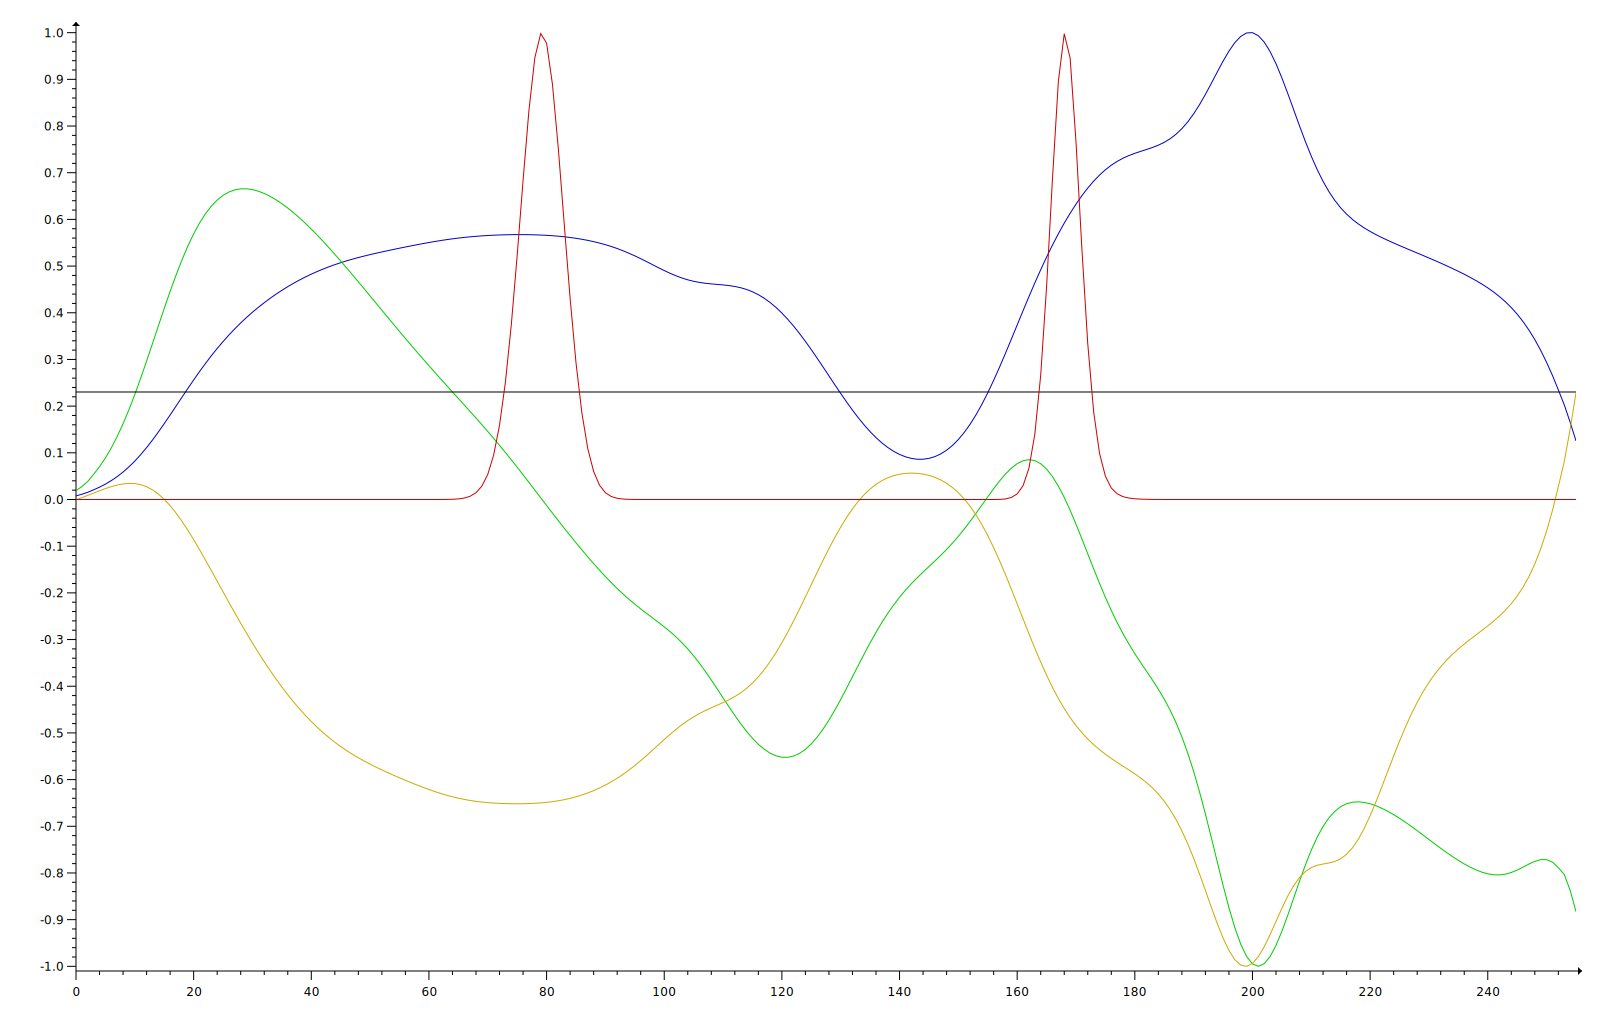
\includegraphics[width=0.35\textwidth]{images/r_g_engine}
		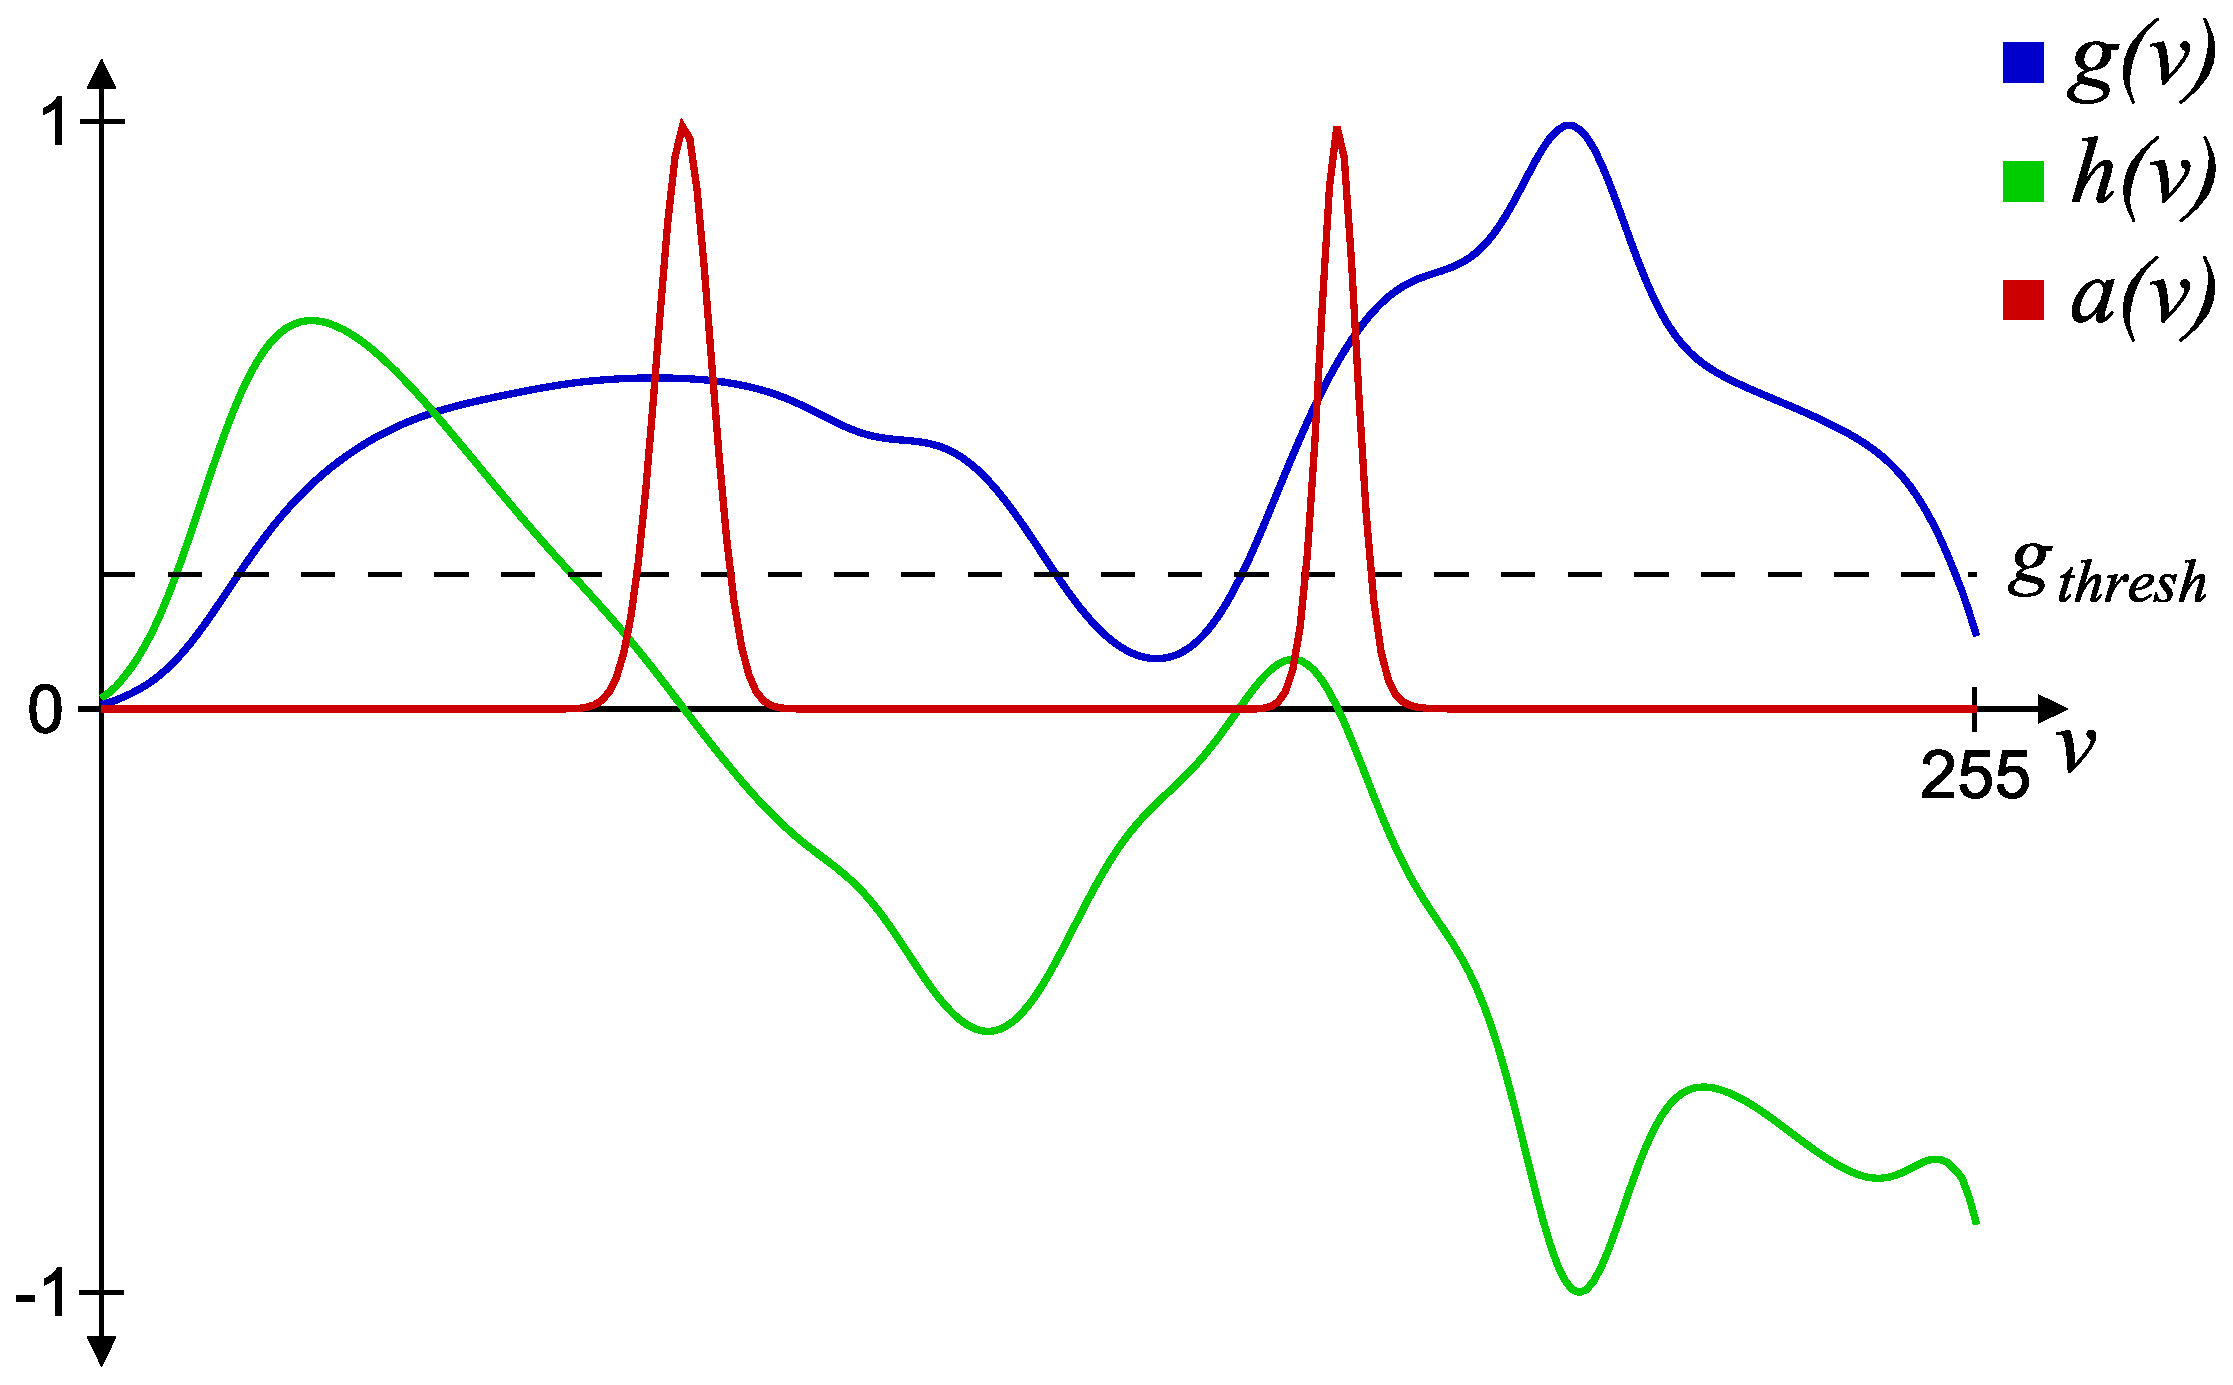
\includegraphics[width=0.65\textwidth]{images/r_g_engine_ft}
		\label{fig:r_engine_kd}
	}
	\subfigure[Método proposto.]
	{
		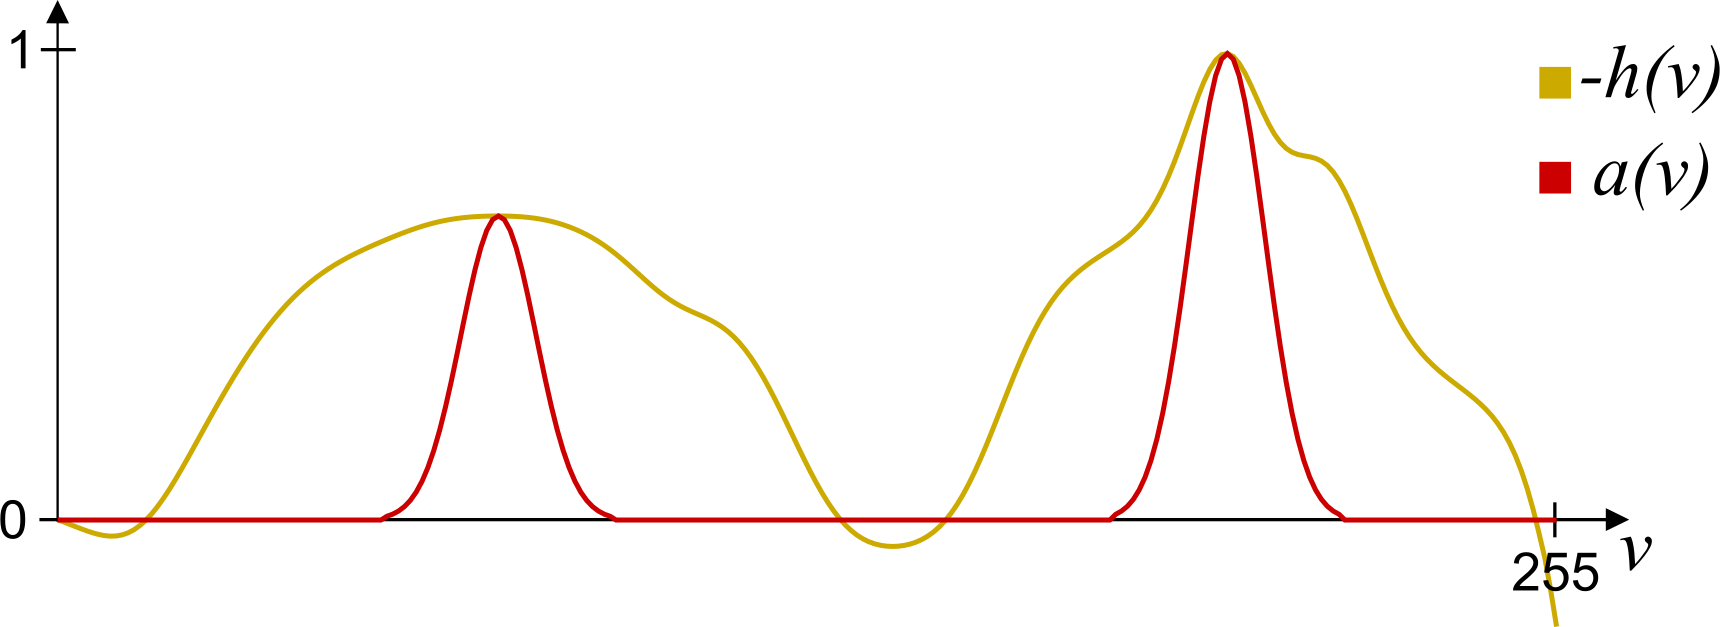
\includegraphics[width=0.35\textwidth]{images/r_m_engine}
		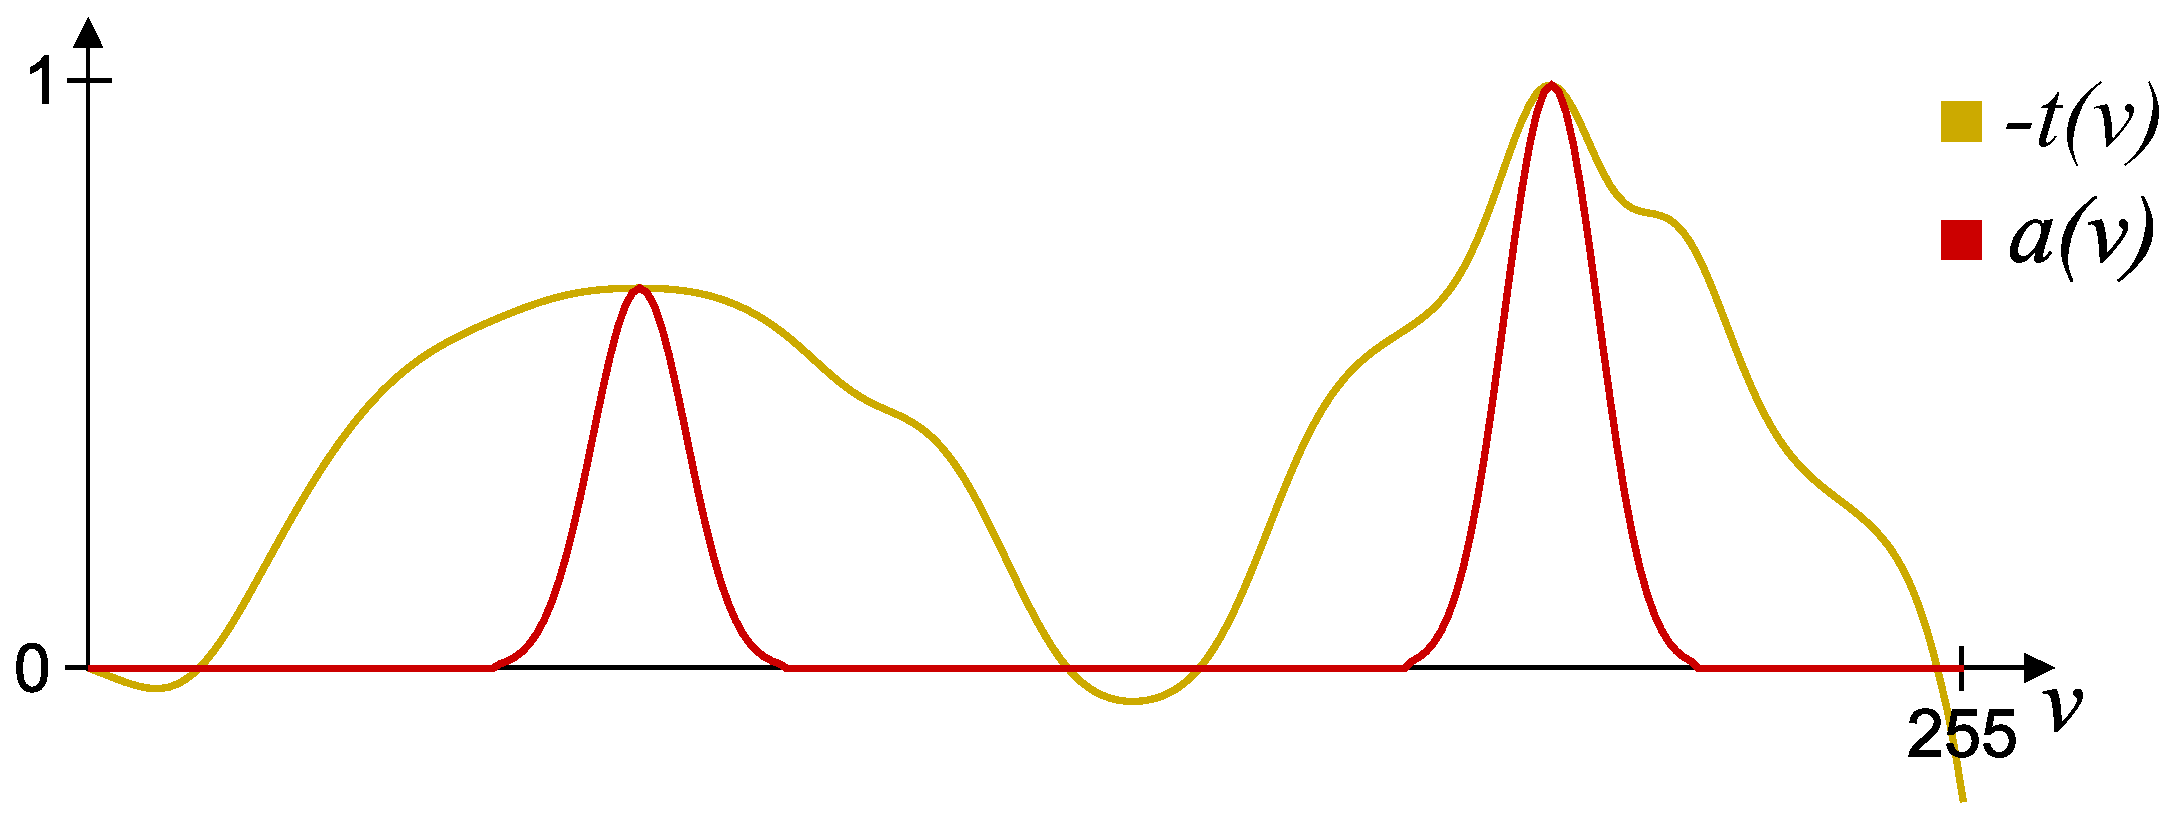
\includegraphics[width=0.65\textwidth]{images/r_m_engine_ft}			\label{fig:r_engine_mine}
	}
	\caption{Visualização e função de transferência do volume \quote{Engine}.}
	\label{fig:r_engine}
\end{figure}

A Figura~\ref{fig:r_engine_slice} exibe uma fatia do volume \quote{Engine}, onde pode ser observada a existência de $ 3 $ fronteiras. Comparando as visualizações resultantes dos dois métodos, exibidas na Figura~\ref{fig:r_engine}, percebe-se que ambos foram capazes de realçar corretamente as fronteiras do volume. No entanto, ressalta-se que esta equivalência só foi possível após encontrar o valor de $ g_{thresh} $ que eliminou algumas regiões da visualização do método de \textit{Kindlmann e Durkin} que foram realçadas indevidamente, devido ao deslocamento do segundo pico da sua função de transferência.
\clearpage
%%%%%%%%%%%%%%%%%%%%%%%%%%%%%%%%%% CT HEAD %%%%%%%%%%%%%%%%%%%%%%%%%%%%%%%%%%%%%
\begin{figure}[h]
	\centering
	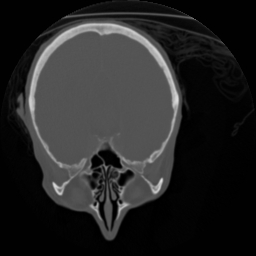
\includegraphics[width=0.3\textwidth]{images/r_cthead_slice}
	\caption{Fatia do volume \quote{CT Head}.}
	\label{fig:r_cthead_slice}
\end{figure}

\begin{figure}[h]
	\centering
	\subfigure[Método de \textit{Kindlmann e Durkin}.]
	{
		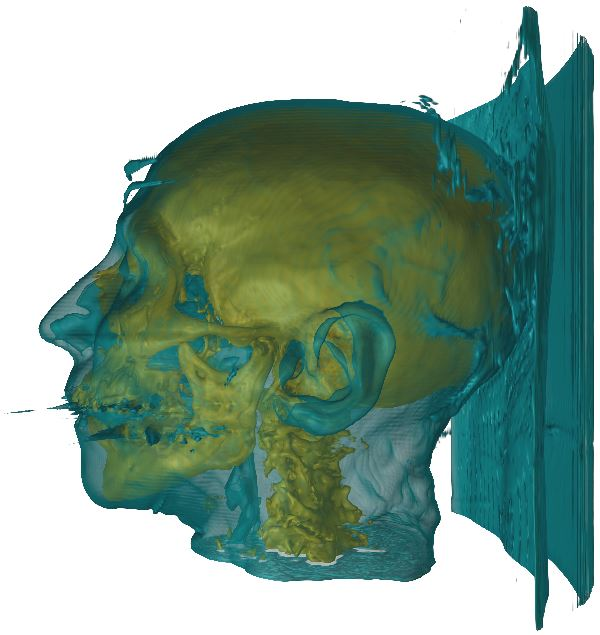
\includegraphics[width=0.35\textwidth]{images/r_g_cthead}
		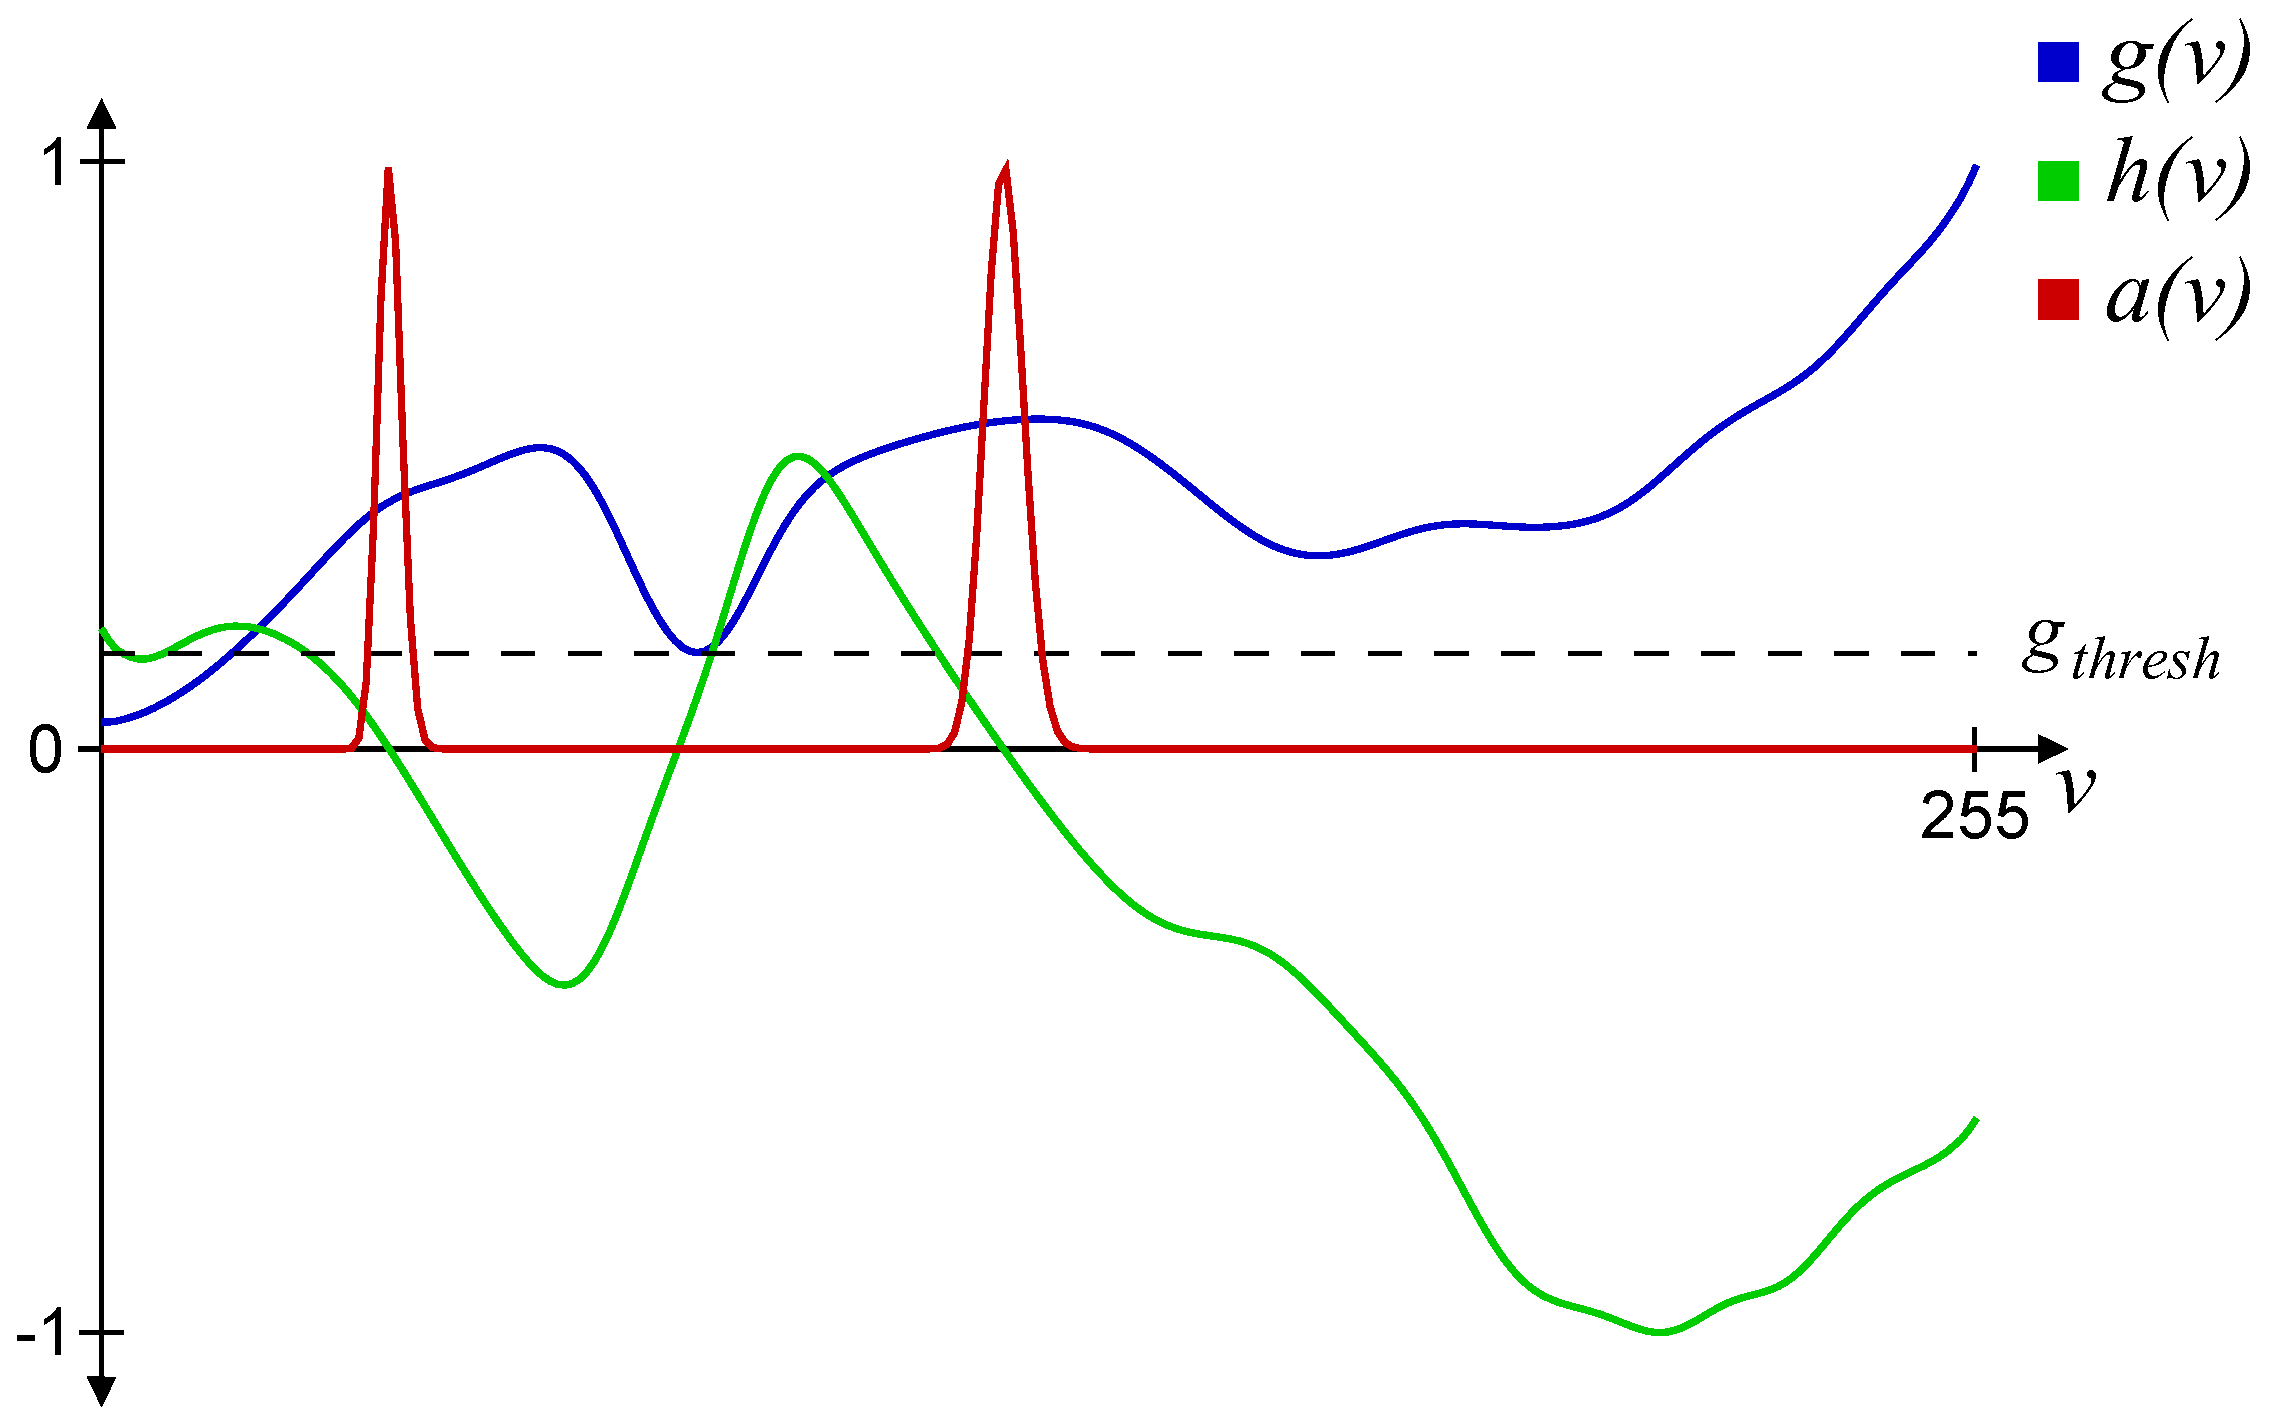
\includegraphics[width=0.65\textwidth]{images/r_g_cthead_ft}
		\label{fig:r_cthead_kd}
	}
	\subfigure[Método proposto.]
	{
		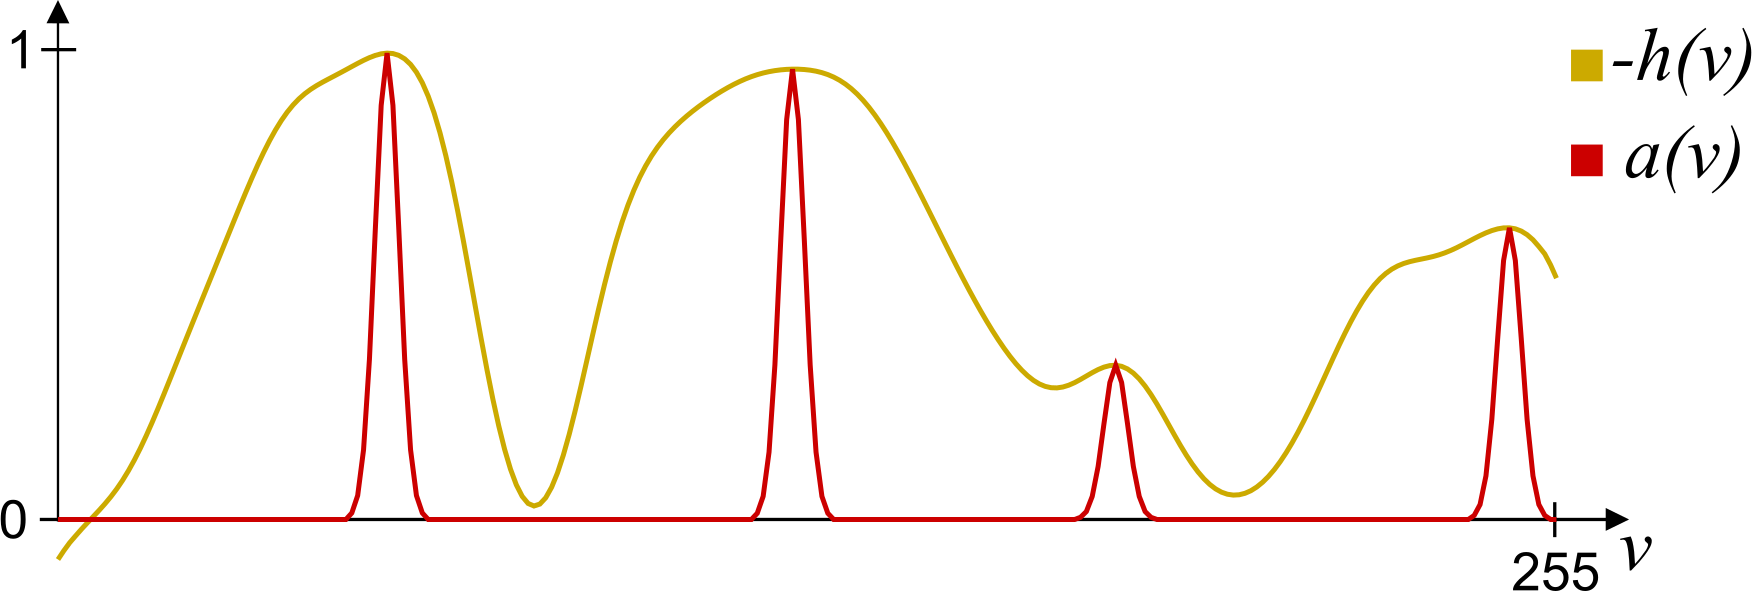
\includegraphics[width=0.35\textwidth]{images/r_m_cthead}
		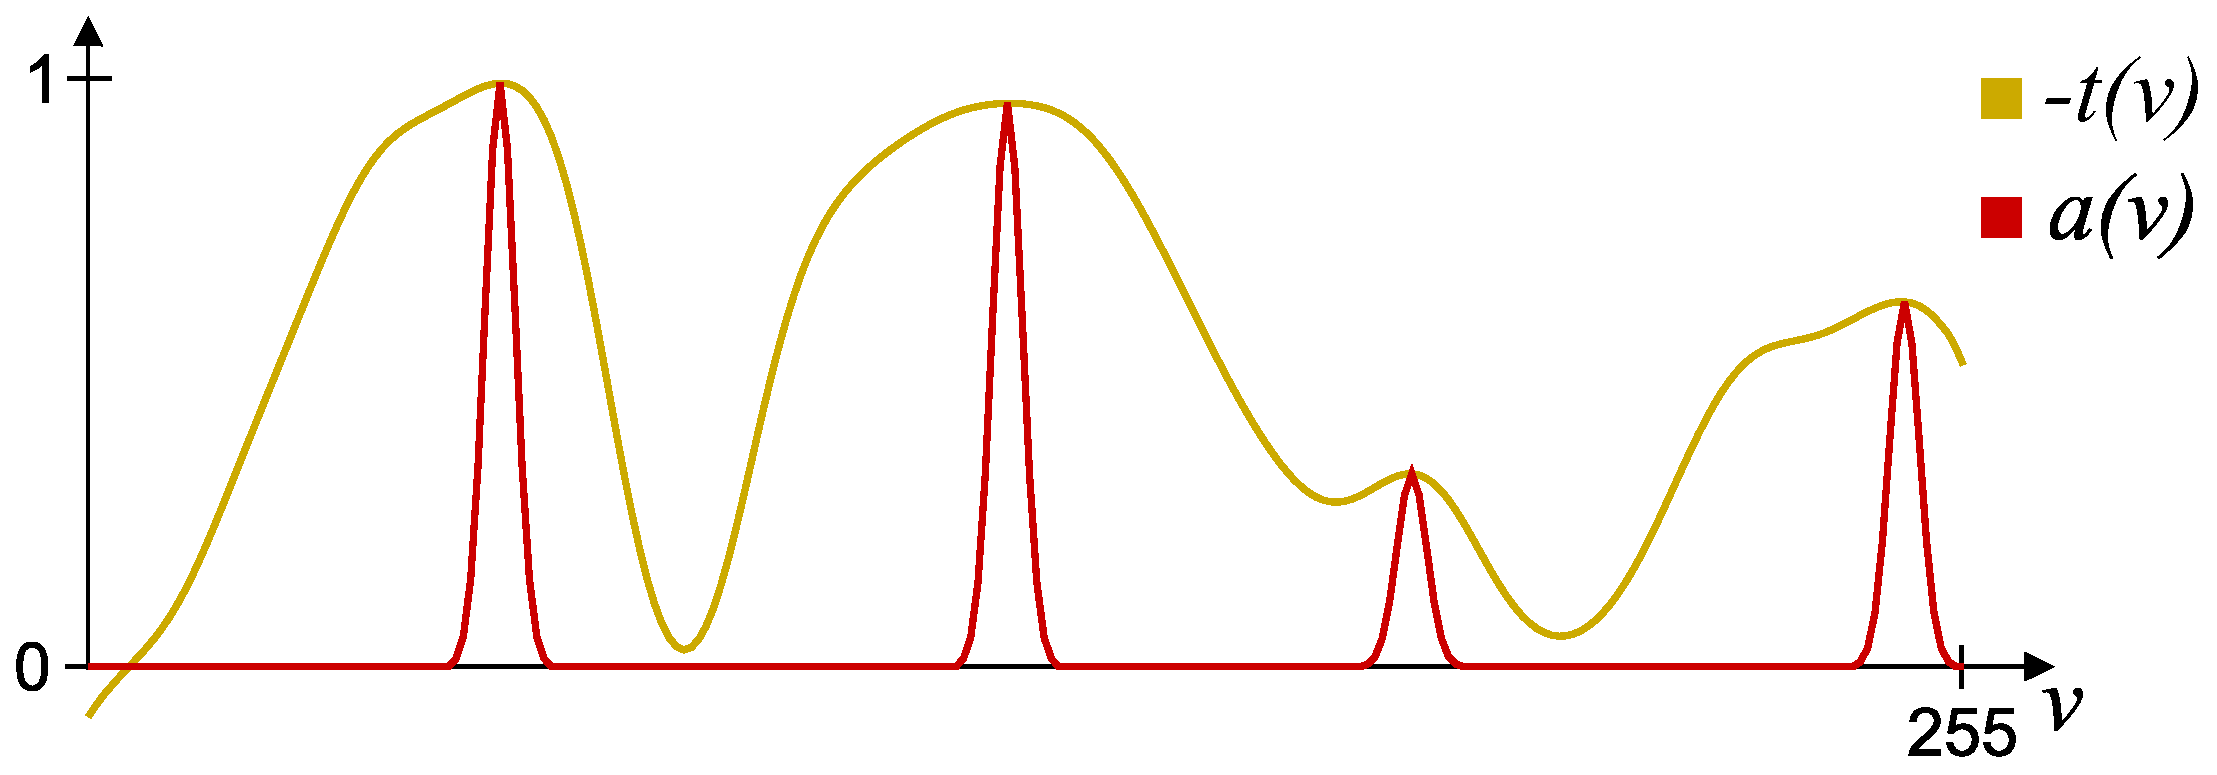
\includegraphics[width=0.65\textwidth]{images/r_m_cthead_ft}			\label{fig:r_cthead_mine}
	}
	\caption{Visualização e função de transferência do volume \quote{CT Head}.}
	\label{fig:r_cthead}
\end{figure}

	A Figura~\ref{fig:r_cthead_slice} apresenta uma fatia do volume \quote{CT Head}. Como pode ser observado, na parte de trás da cabeça do indivíduo, há uma estrutura que se comporta como uma fronteira. O método de \textit{Kindlmann e Durkin} realçou corretamente a cabeça e o crânio do indivíduo, bem como a estrutura comentada, como ilustra a Figura~\ref{fig:r_cthead}~\ref{fig:r_cthead_kd}. Jà o método proposto por esta dissertação foi capaz de realçar corretamente as fronteiras do indivíduo, porém, mostrando menos a estrutura presente na parte de trás. Este resultado, exibido na Figura~\ref{fig:r_cthead}~\ref{fig:r_cthead_mine} proporciona uma visualização mais limpa e, portanto, facilita ainda mais a compreensão do volume.

	Abaixo são exibidas as visualizações de alguns outros volumes conhecidos:
	
\begin{figure}[H]
	\centering
	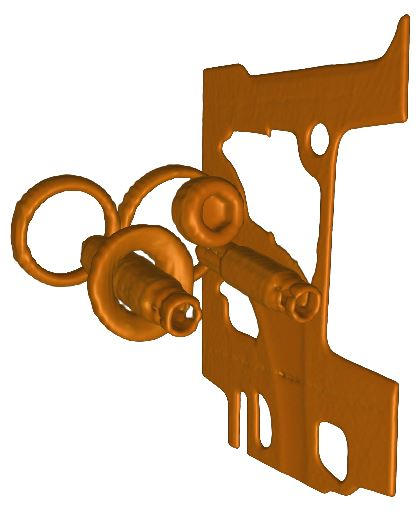
\includegraphics[width=0.5\textwidth]{images/r_m_engine_iso}
	\caption{Estrutura interna do volume \quote{Engine}.}
\end{figure}

\begin{figure}[H]
	\centering
	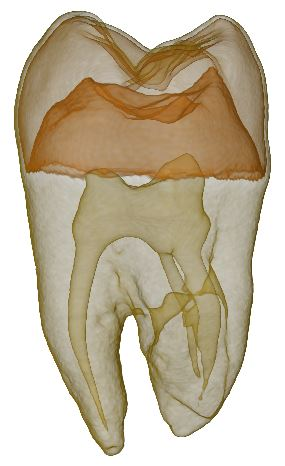
\includegraphics[width=0.4\textwidth]{images/r_m_tooth}
	\caption{\quote{Tooth}.}
\end{figure}

\begin{figure}[H]
	\centering
	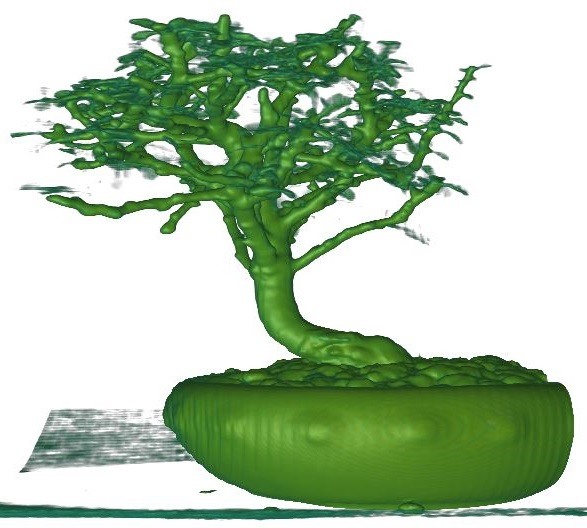
\includegraphics[width=0.8\textwidth]{images/r_m_bonsai}
	\caption{\quote{Bonsai}.}
\end{figure}

\begin{figure}[H]
	\centering
	\subfigure
	{
		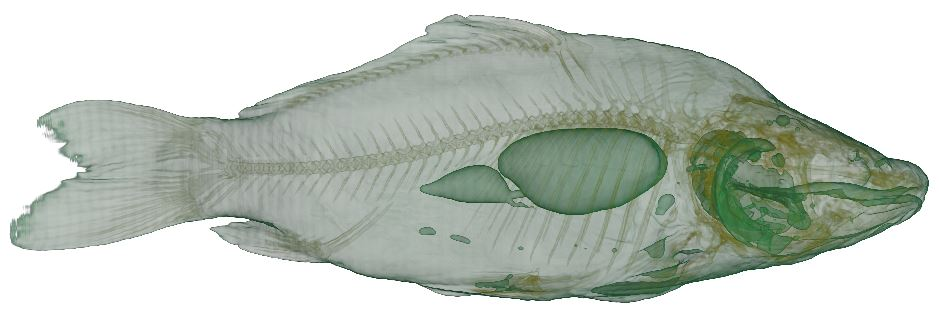
\includegraphics[width=0.7\textwidth]{images/r_m_carp}
	}
	\subfigure
	{
		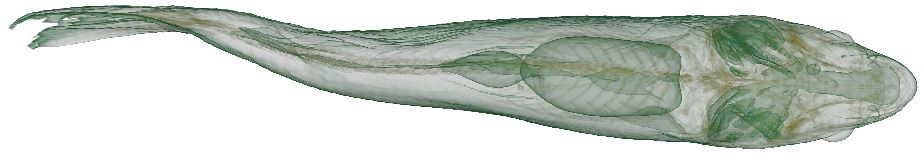
\includegraphics[width=0.7\textwidth]{images/r_m_carp_up}
	}
	\subfigure
	{
		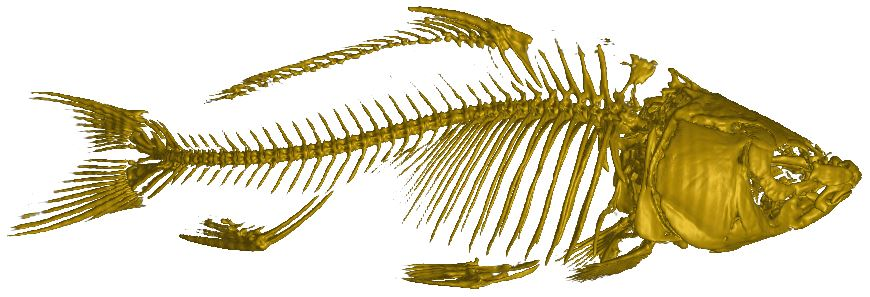
\includegraphics[width=0.7\textwidth]{images/r_m_carp_exo}
	}
	\caption{\quote{Carp}.}
\end{figure}

\begin{figure}[H]
	\centering
	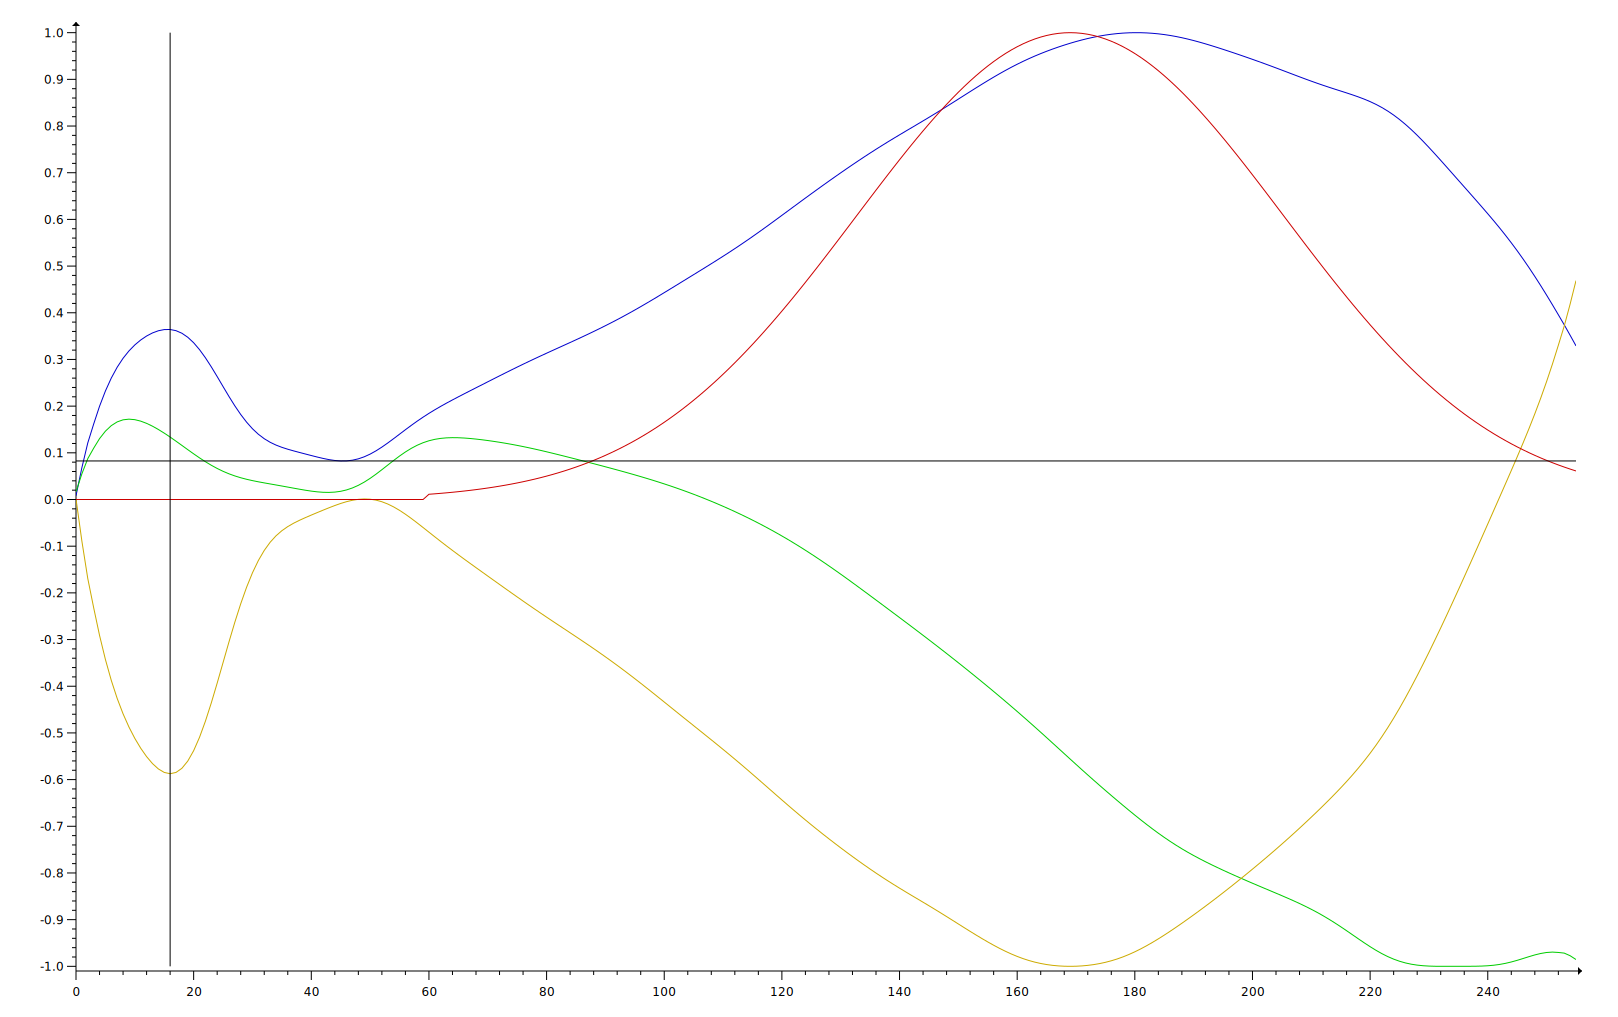
\includegraphics[width=0.7\textwidth]{images/r_m_knee}
	\caption{\quote{Knee}.}
\end{figure}

\section{Malhas Não Regulares}
\label{sec:result.irreg}

	Para visualizar volumes com malhas não regulares foi preciso utilizar um outro visualizador. Escolheu-se então a técnica proposta por \textit{Miranda e Celes}~\cite{miranda} em \quote{Accurate volume rendering of unstructed hexahedral meshes}. Como esse método não faz uso de um modelo de iluminação, nota-se uma grande diferença na visualização dos volumes, se comparados com os anteriores. No entanto, a análise dos resultados não é prejudicada.
	
%%%%%%%%%%%%%%%%%%%%%%%%%%%%%%%%% VREP SO 1 %%%%%%%%%%%%%%%%%%%%%%%%%%%%%%%%%%%%
\begin{figure}[h]
	\centering
	\subfigure[]{
		\frame{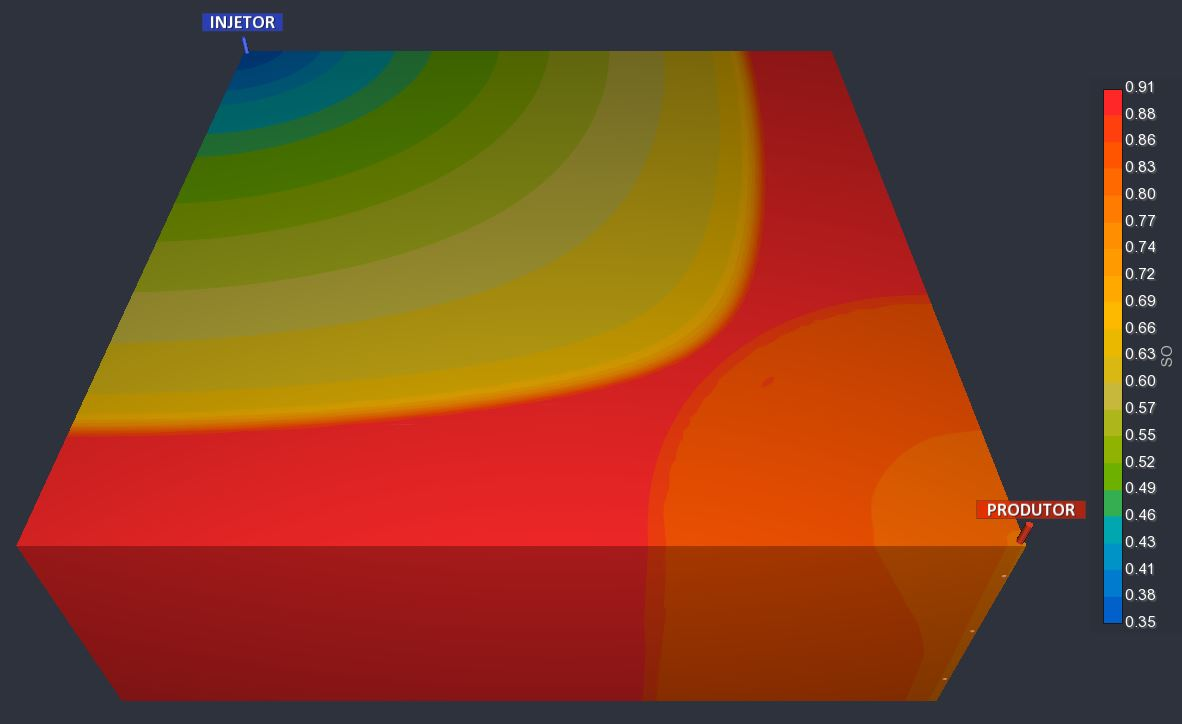
\includegraphics[width=0.3\textwidth]{images/r_vrep_so_slice}}
	}
	\caption{Fatia de um reservatório de petróleo cúbico.}
	\label{fig:box_slice}
\end{figure}

	A figura acima mostra uma fatia da simulação de um reservatório de petróleo cúbico com um poço injetor no canto superior esquerdo e um produtor no canto diagonal oposto. A propriedade simulada é saturação de óleo.

\begin{figure}[h]
	\centering
	\subfigure[Método de \textit{Kindlmann e Durkin}.]
	{
		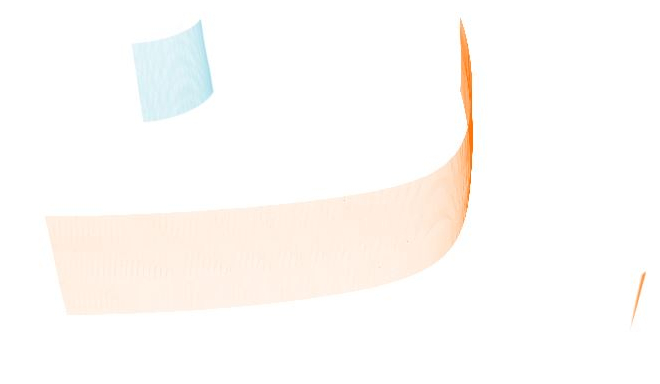
\includegraphics[width=0.35\textwidth]{images/r_vrep_so_kd}
		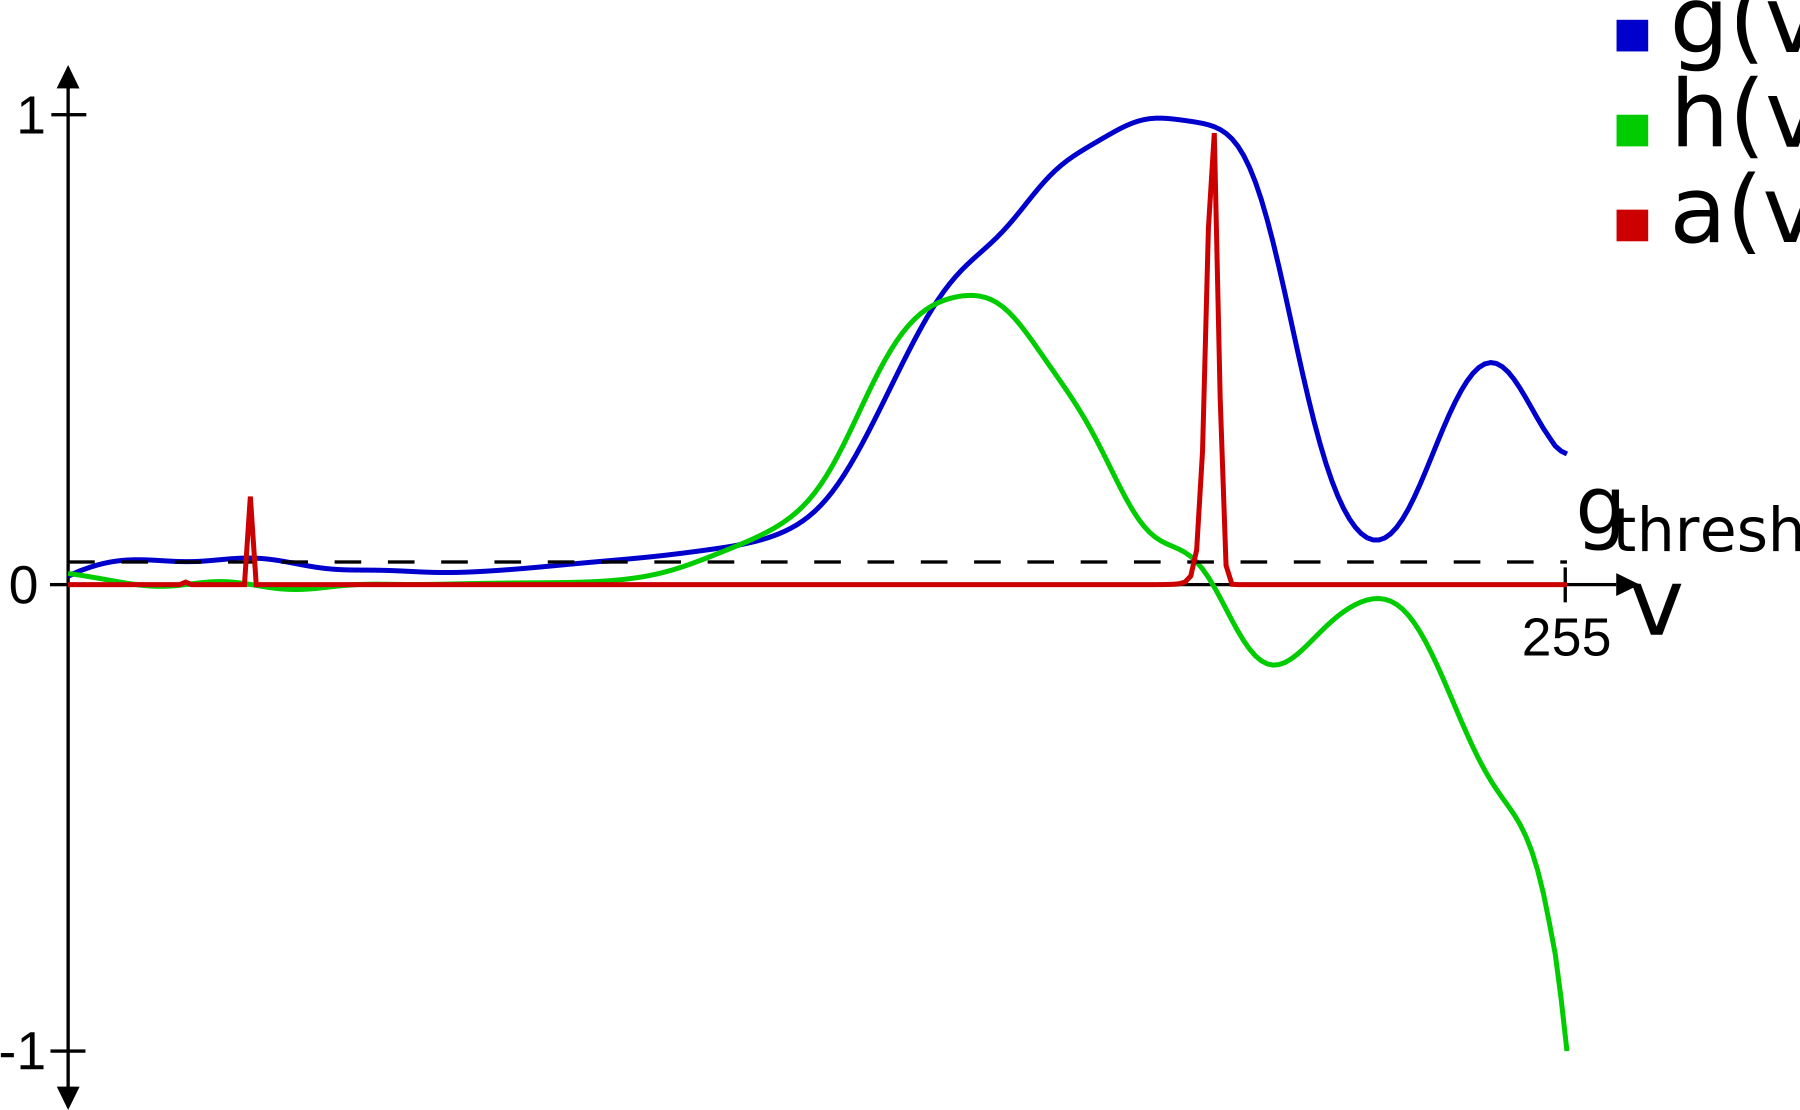
\includegraphics[width=0.65\textwidth]{images/r_vrep_so_kd_ft}
		\label{fig:r_vrep_kd}
	}
	\subfigure[Método proposto.]
	{
		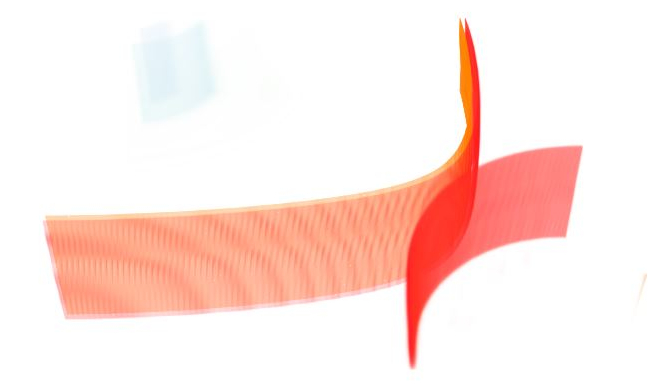
\includegraphics[width=0.35\textwidth]{images/r_vrep_so_mine}
		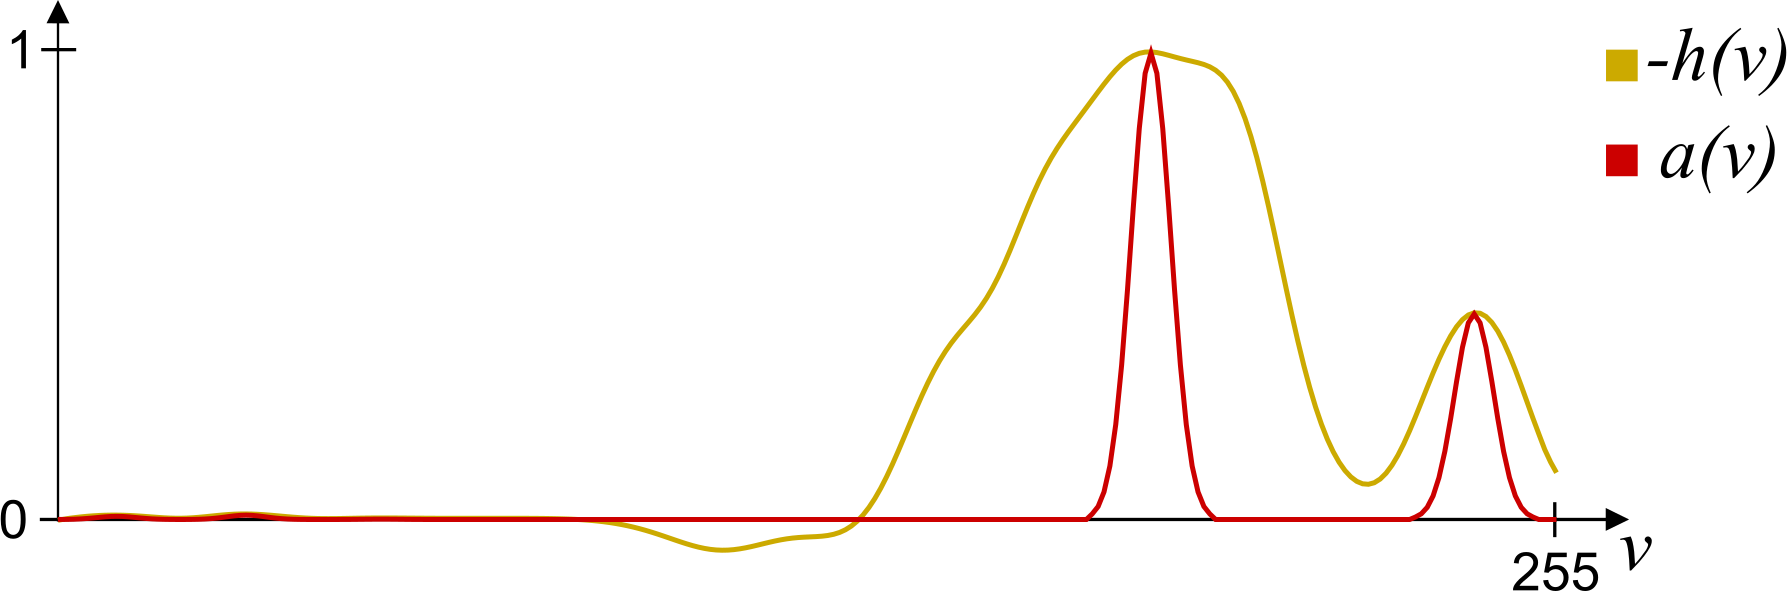
\includegraphics[width=0.65\textwidth]{images/r_vrep_so_mine_ft}			\label{fig:r_vrep_mine}
	}
	\caption{Visualização e função de transferência do reservatório de petróleo cúbico.}
	\label{fig:r_vrep}
\end{figure}

	Como pode ser visto na Figura~\ref{fig:box_slice}, o reservatório possui duas fronteiras bem destacadas e uma mais fraca que são, respectivamente: cinza escuro-branco, branco-cinza claro e preto-cinza escuro. A Figura~\ref{fig:r_vrep} mostra que o método de \textit{Kindlmann e Durkin} identifica apenas a primeira e a terceira das fronteiras listadas, reforçando o quanto essa abordagem é dependente de $ h(v) = 0 $. Já o método descrito por esta dissertação identifica uma fronteira fraca a mais que o esperado. Porém, realça corretamente as duas mais fortes.

%%%%%%%%%%%%%%%%%%%%%%%%%%%%%%%%% VREP SO 2 %%%%%%%%%%%%%%%%%%%%%%%%%%%%%%%%%%%%
\begin{figure}[h]
	\centering
	\frame{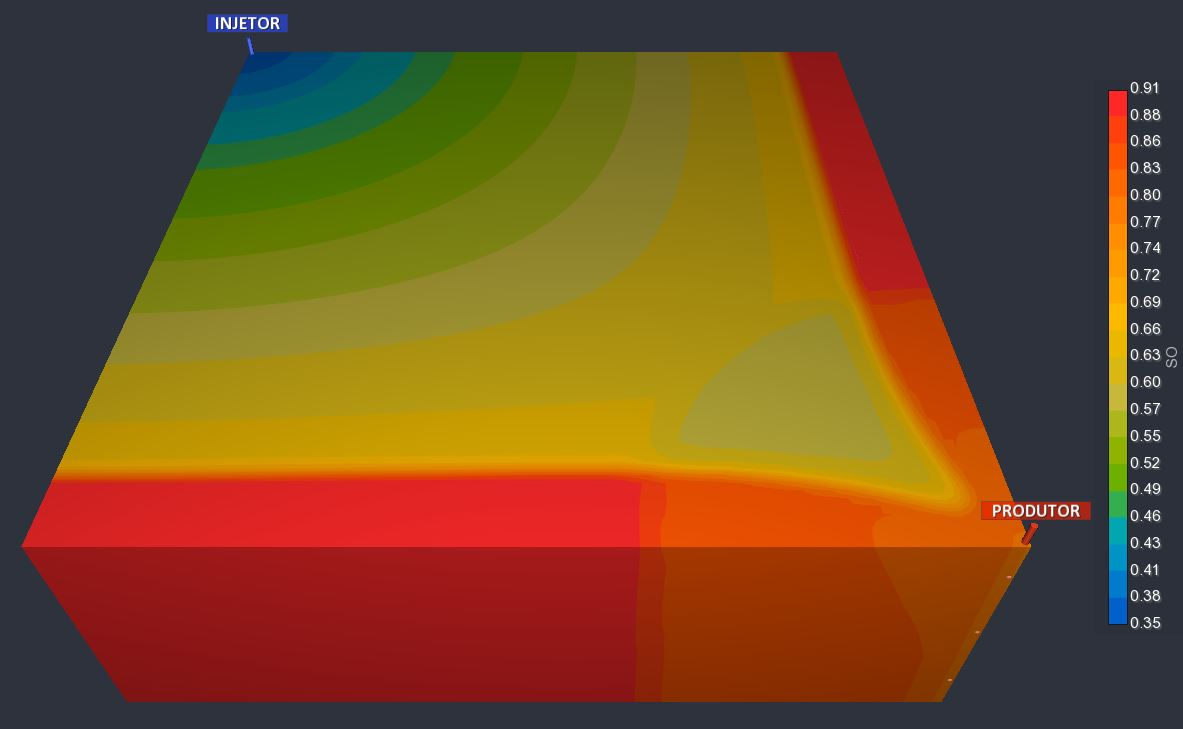
\includegraphics[width=0.3\textwidth]{images/r_vrep_so_2_slice}}
	\caption{Fatia de um reservatório de petróleo cúbico.}
\end{figure}

	A figura acima refere-se ao mesmo volume da Figura~\ref{fig:box_slice}, mas em outro momento da simulação. Agora há apenas uma fronteira forte: aquela que divide a região escura da região clara, na fatia do volume. Contudo, três fronteiras mais fracas ainda podem ser vistas.

\begin{figure}[h]
	\centering
	\subfigure[Método de \textit{Kindlmann e Durkin}.]
	{
		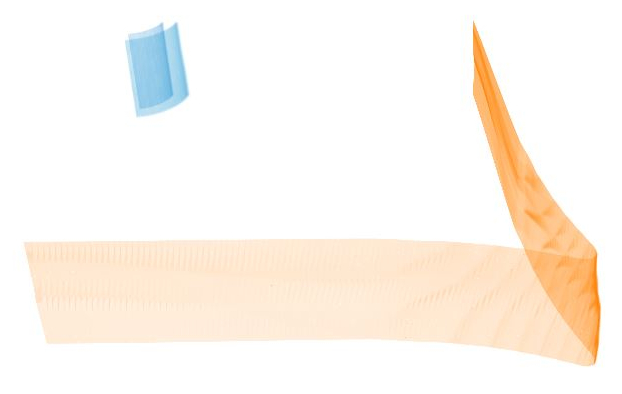
\includegraphics[width=0.35\textwidth]{images/r_vrep_so_2_kd}
		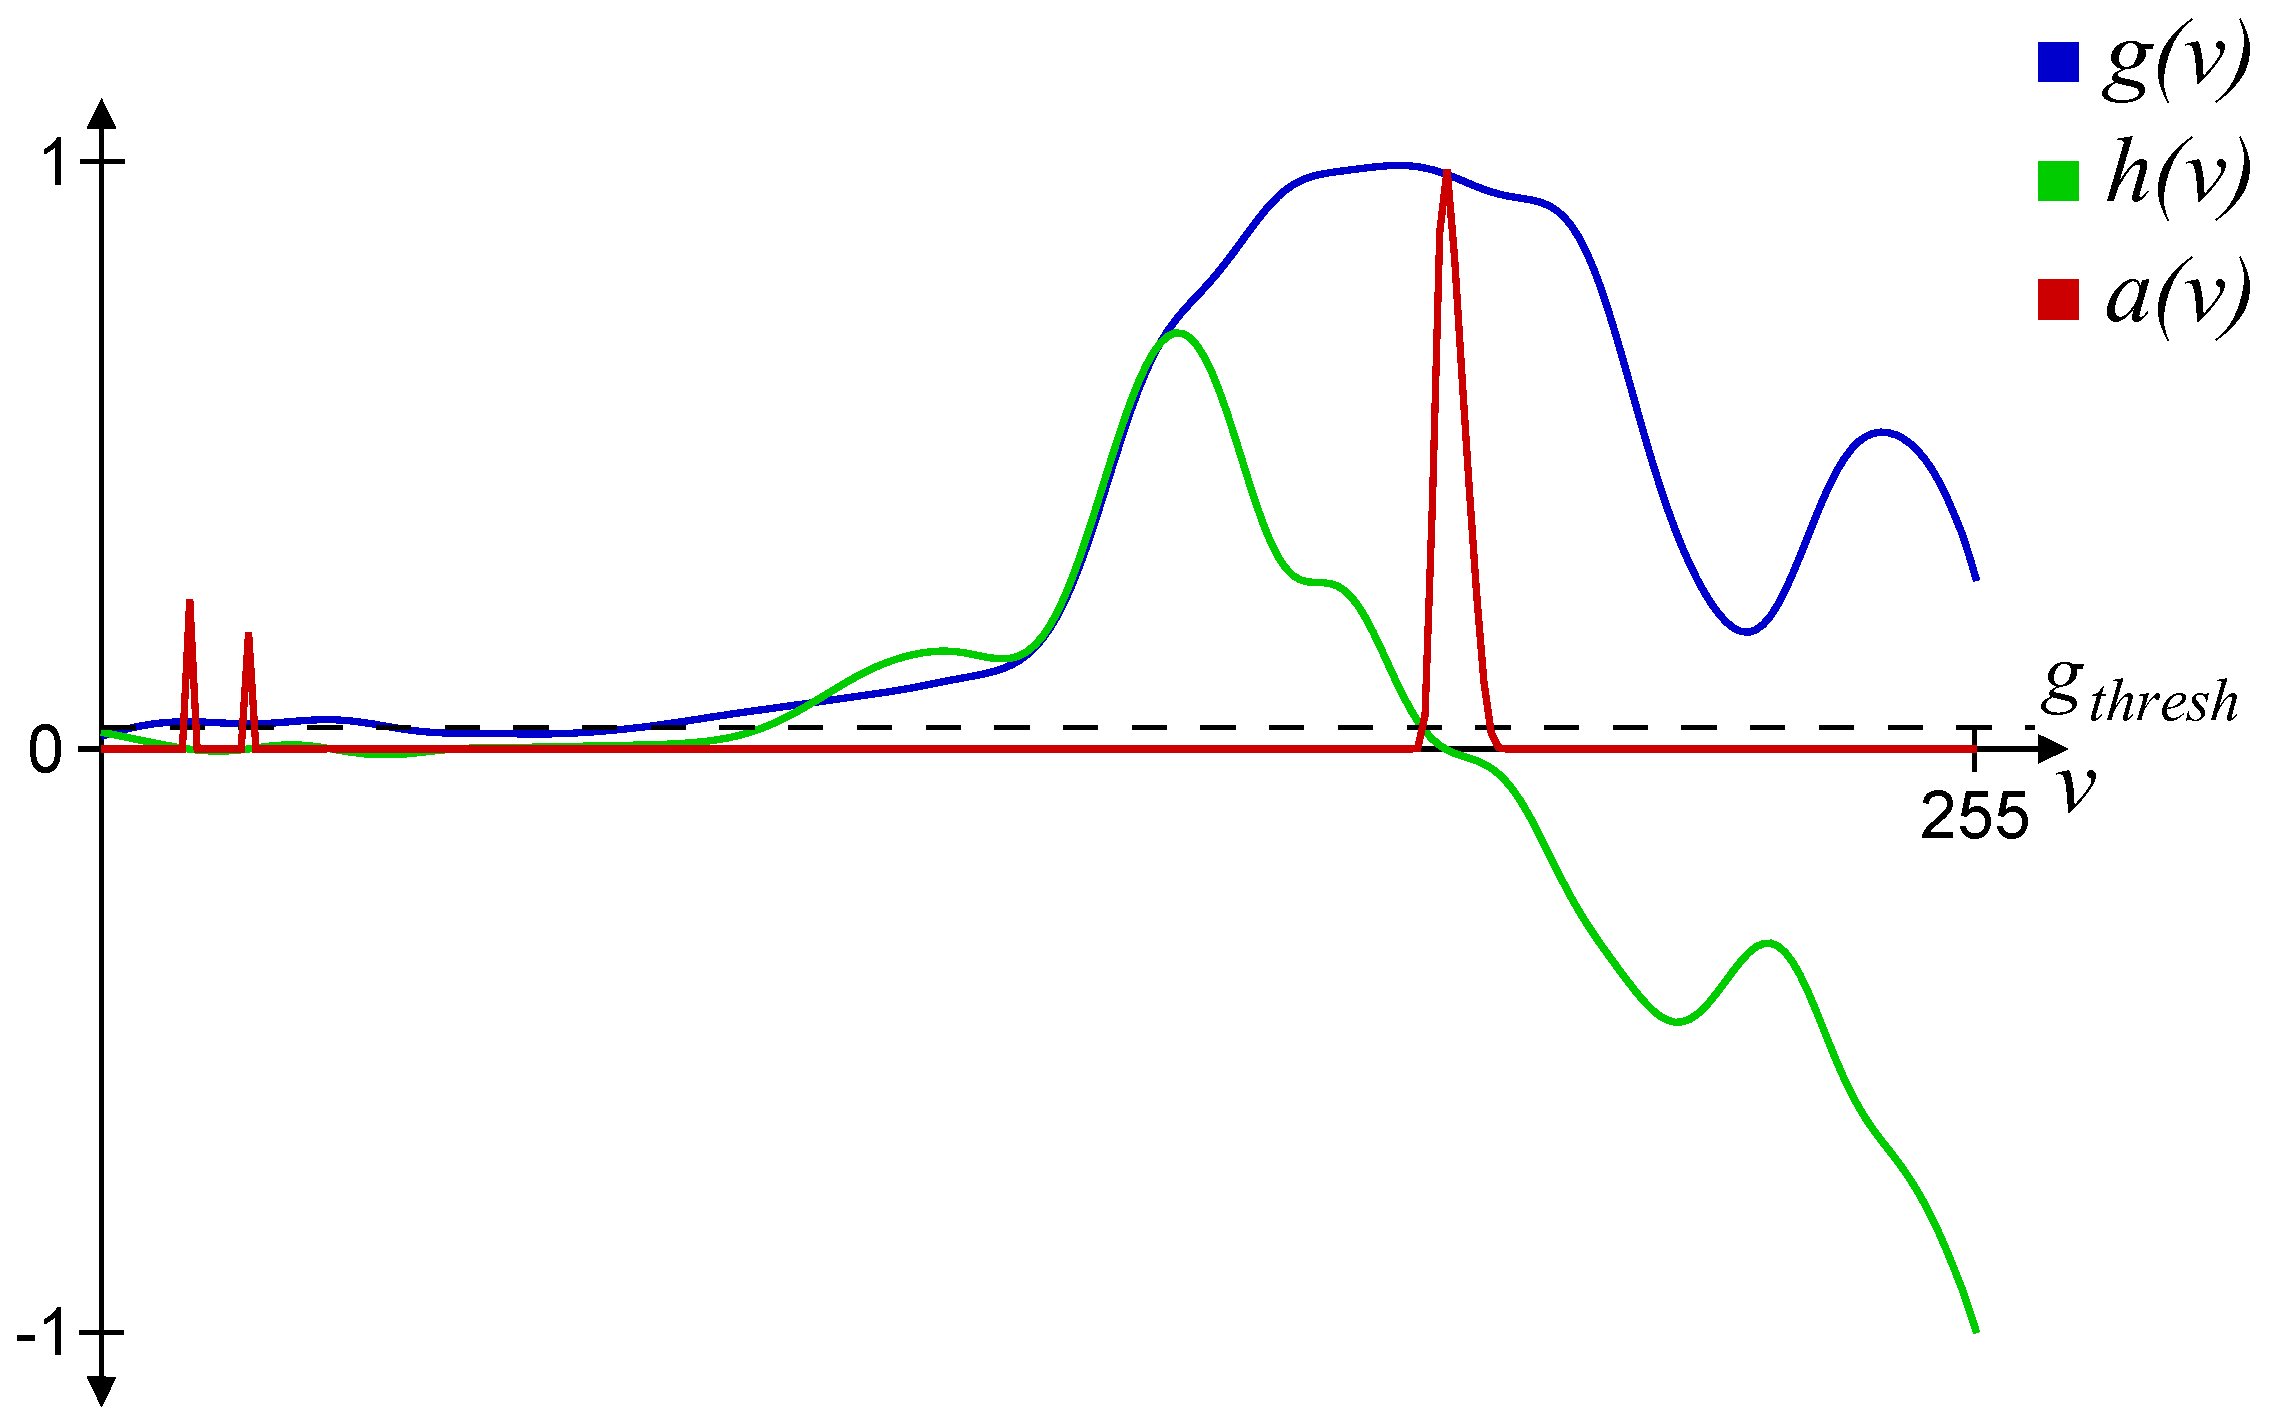
\includegraphics[width=0.65\textwidth]{images/r_vrep_so_2_kd_ft}
		\label{fig:r_vrep_2_kd}
	}
	\subfigure[Método proposto.]
	{
		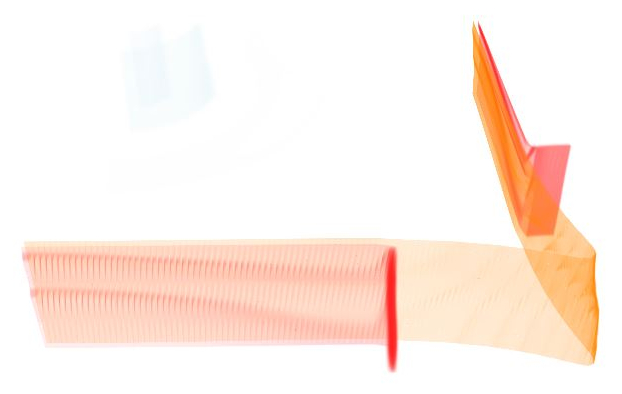
\includegraphics[width=0.35\textwidth]{images/r_vrep_so_2_mine}
		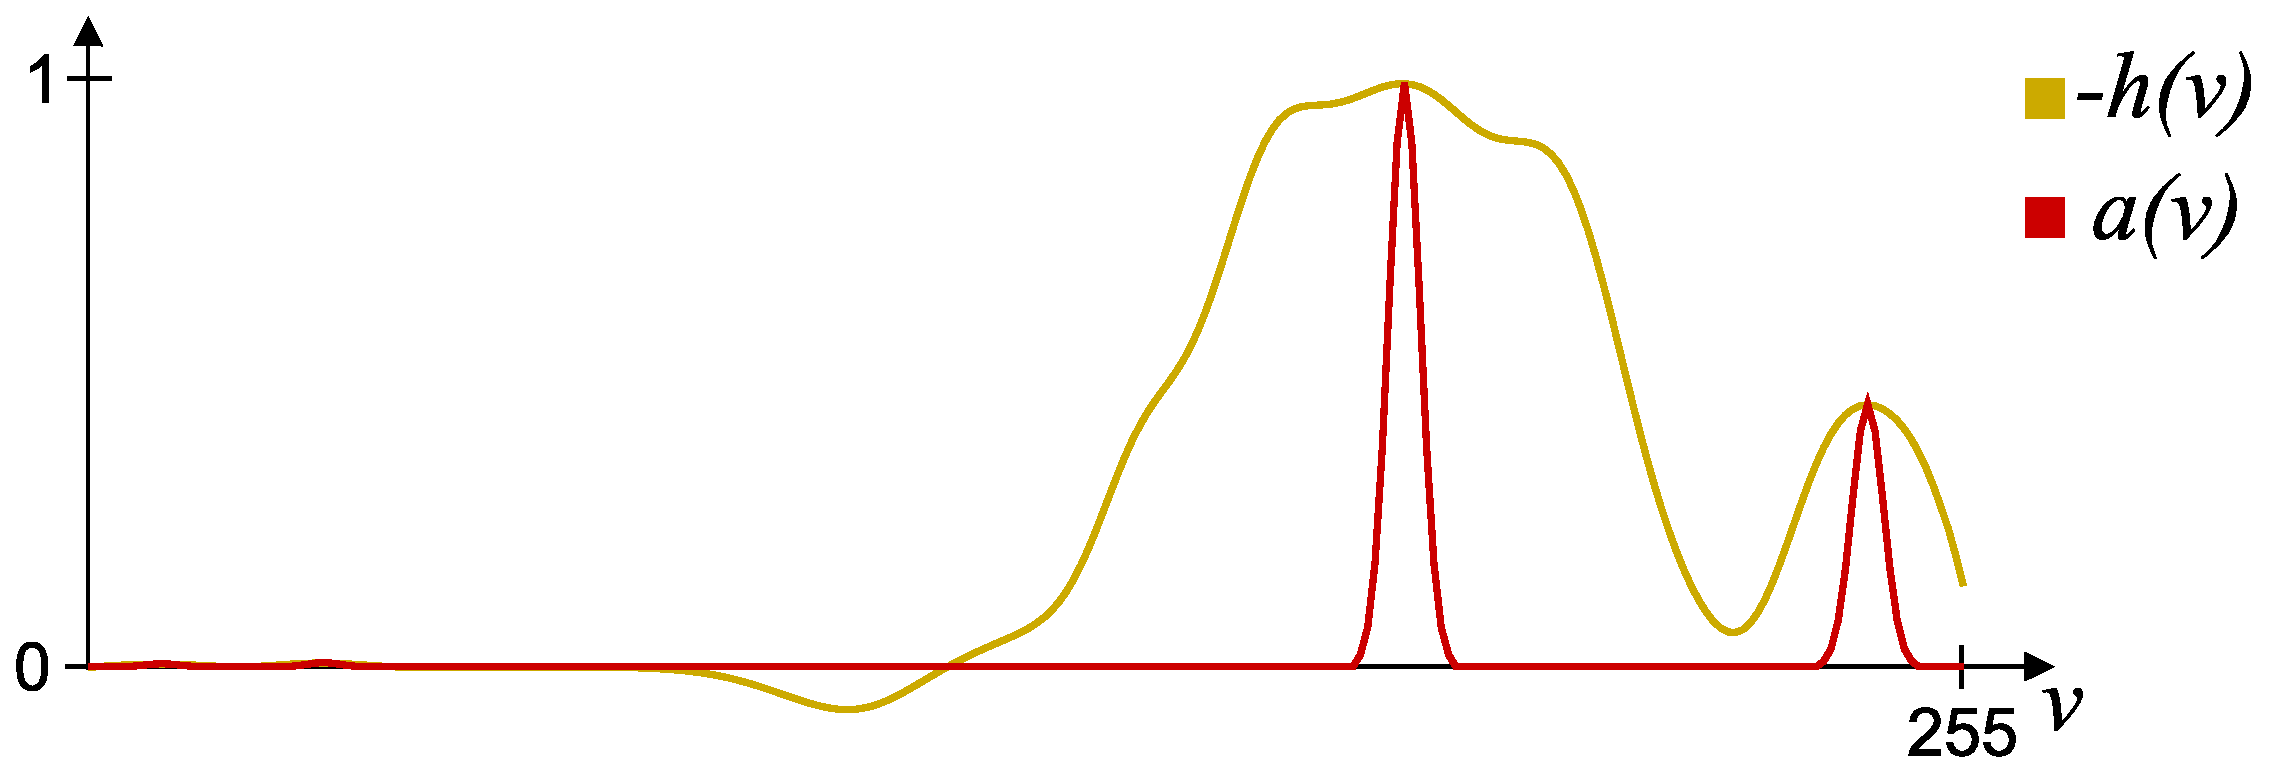
\includegraphics[width=0.65\textwidth]{images/r_vrep_so_2_mine_ft}			\label{fig:r_vrep_2_mine}
	}
	\caption{Visualização e função de transferência do reservatório de petróleo cúbico.}
	\label{fig:r_vrep_2}
\end{figure}

	Como mostra a Figura~\ref{fig:r_vrep_2} acima, nenhum método foi capaz de realçar todas as fronteiras. Utilizando \textit{Kindlmann e Durkin} obteve-se as fronteiras $ 1 $ e $ 4 $ enquanto com o método proposto nesta dissertação obteve-se as fronteiras $ 1 $, $ 3 $ e $ 4 $. O motivo pelo qual $ 4 $ é realçada com opacidade muito baixa é a estreita relação entre opacidade e amplitude de $ -h(v) $.
	
%%%%%%%%%%%%%%%%%%%%%%%%%%%%%%%%%% BOX SO %%%%%%%%%%%%%%%%%%%%%%%%%%%%%%%%%%%%%
\begin{figure}[h]
	\centering
	\frame{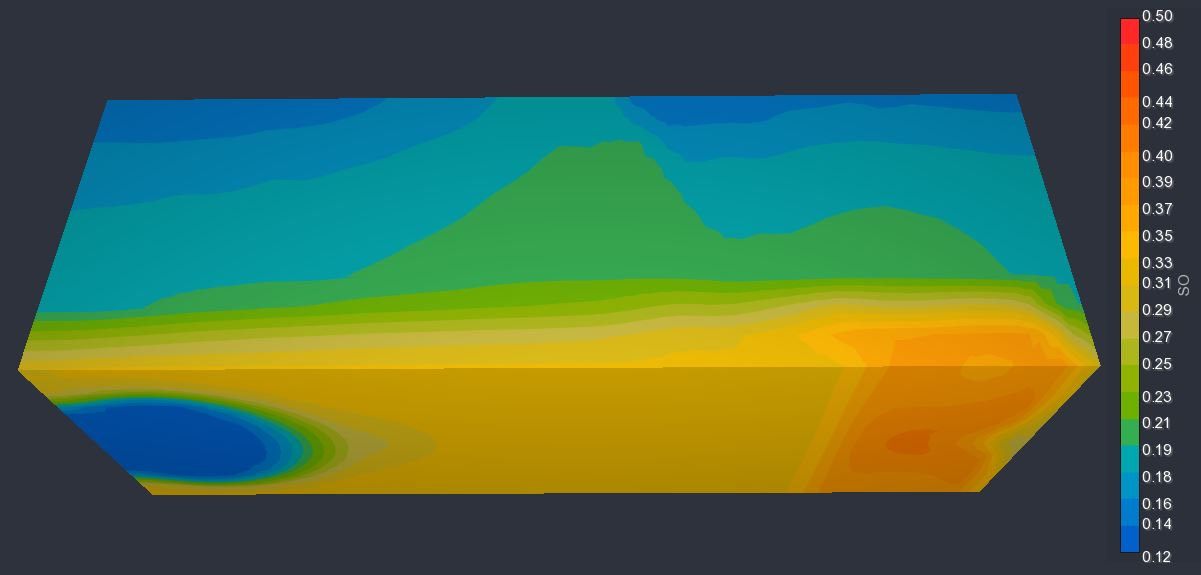
\includegraphics[width=0.5\textwidth]{images/r_box_so_slice}}
	\caption{Fatia do volume \quote{Caixa de sapato} com a propriedade saturação de óleo.}
\end{figure}

	A figura acima mostra uma fatia da simulação de um reservatório de petróleo retangular com um poço injetor à superior e um produtor à direita, chamado \quote{Caixa de sapato}. A propriedade simulada é saturação de óleo.

\begin{figure}[h]
	\centering
	\subfigure[Função de transferência pelo método de \textit{Kindlmann e Durkin}.]
	{
		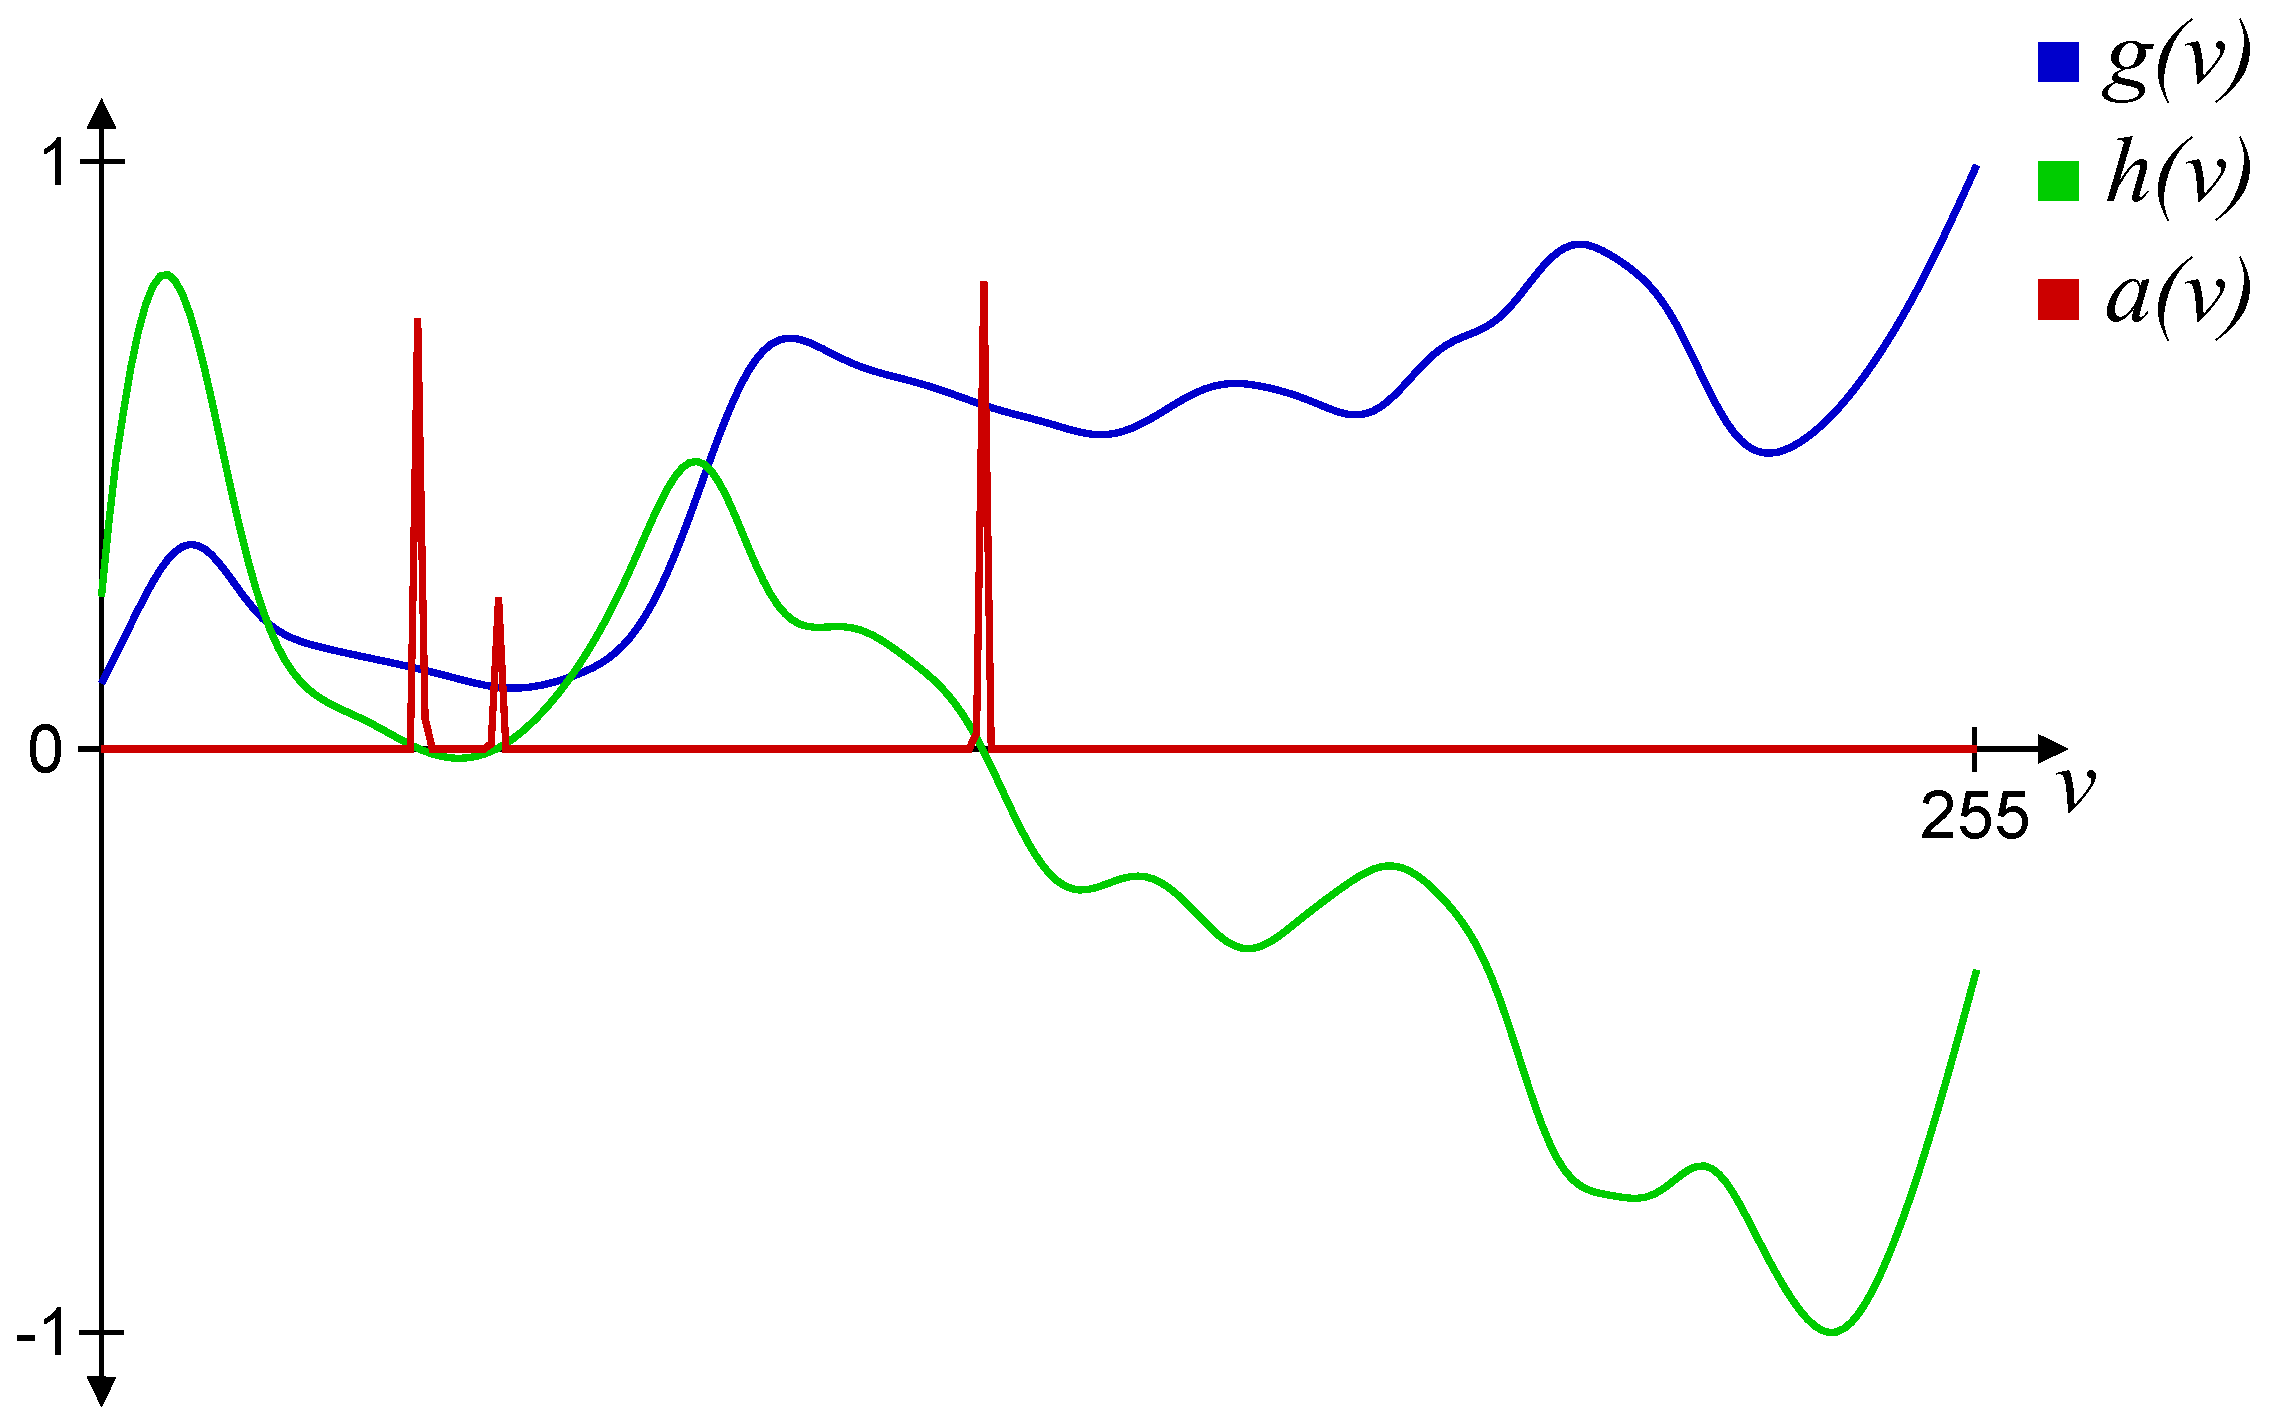
\includegraphics[width=0.7\textwidth]{images/r_box_so_kd_ft}
		\label{fig:r_box_so_kd_ft}
	}
	\subfigure[Visualização pela FT do método de \textit{Kindlmann e Durkin}.]
	{
		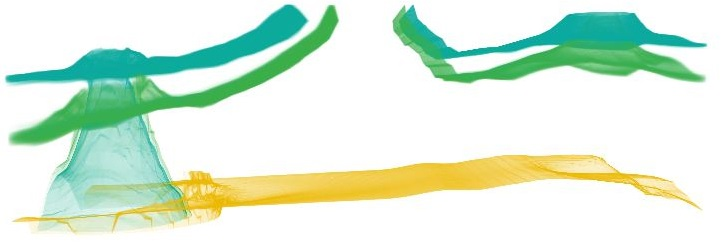
\includegraphics[width=0.7\textwidth]{images/r_box_so_kd}
		\label{fig:r_box_so_kd}
	}
	\subfigure[Função de transferência pelo método proposto.]
	{
		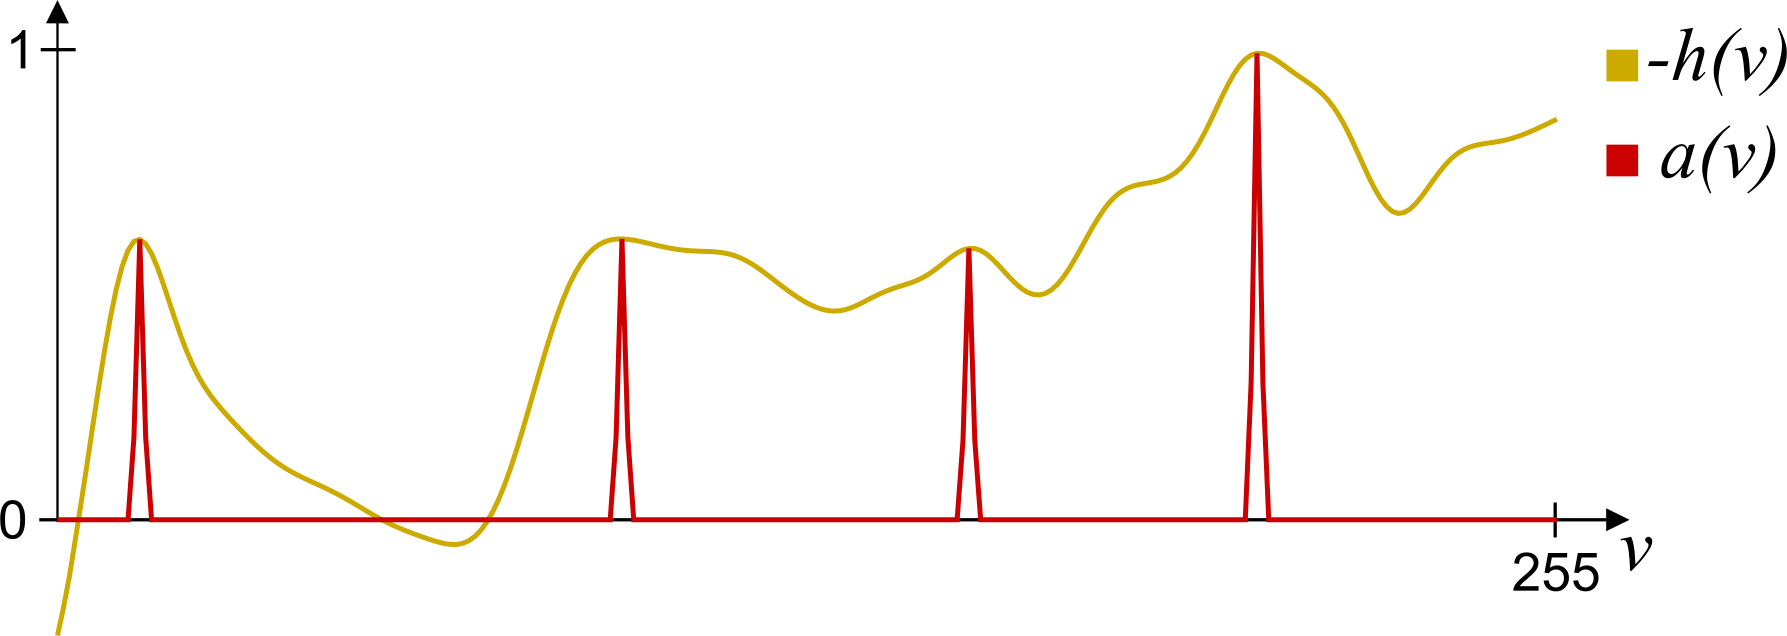
\includegraphics[width=0.7\textwidth]{images/r_box_so_mine_ft}			\label{fig:r_box_so_mine_ft}
	}
	\subfigure[Visualização pela FT do método proposto.]
	{
		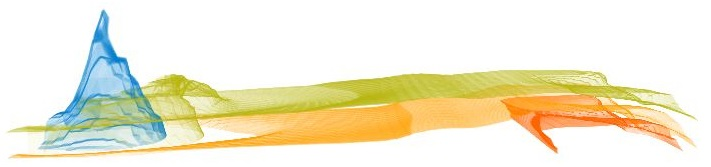
\includegraphics[width=0.7\textwidth]{images/r_box_so_mine}	\label{fig:r_box_so_mine}
	}
	\caption{Visualização e função de transferência do volume \quote{Caixa de sapato} com a propriedade saturação de óleo.}
	\label{fig:r_box_so}
\end{figure}

	No lado esquerdo da fatia do volume em questão é possível perceber um cone, com sua base voltada para baixo. A parte interna do cone é preta e faz fronteira com seu contorno que possui uma tonalidade de cinza claro. Este contorno por sua vez, faz fronteira com o resto do volume em um tom de cinza mais escuro. Então, através da Figura~\ref{fig:r_box_so} observa-se que o método proposto por esta dissertação destaca a fronteira interna do cone (a mais forte), enquanto o método de \textit{Kindlmann e Durkin} realça a fronteira externa do cone.
	
	Como esse volume é pequeno, falta resolução em sua fatia para discutir qual das fronteiras amarelas é a mais adequada. Contudo, pode-se destacar que ambos os métodos destacam fronteiras mais fracas distintas.

%%%%%%%%%%%%%%%%%%%%%%%%%%%%%%%%%% BOX SG %%%%%%%%%%%%%%%%%%%%%%%%%%%%%%%%%%%%%
\begin{figure}[h]
	\centering
	\frame{
\includegraphics[width=0.5\textwidth]{images/r_box_sg_slice}}
	\caption{Fatia do volume \quote{Caixa de sapato} com a propriedade saturação de gás.}
\end{figure}

	A figura acima mostra uma fatia do volume \quote{Caixa de sapato} com a propriedade saturação de gás.

\begin{figure}[h]
	\centering
	\subfigure[Função de transferência pelo método de \textit{Kindlmann e Durkin}.]
	{
		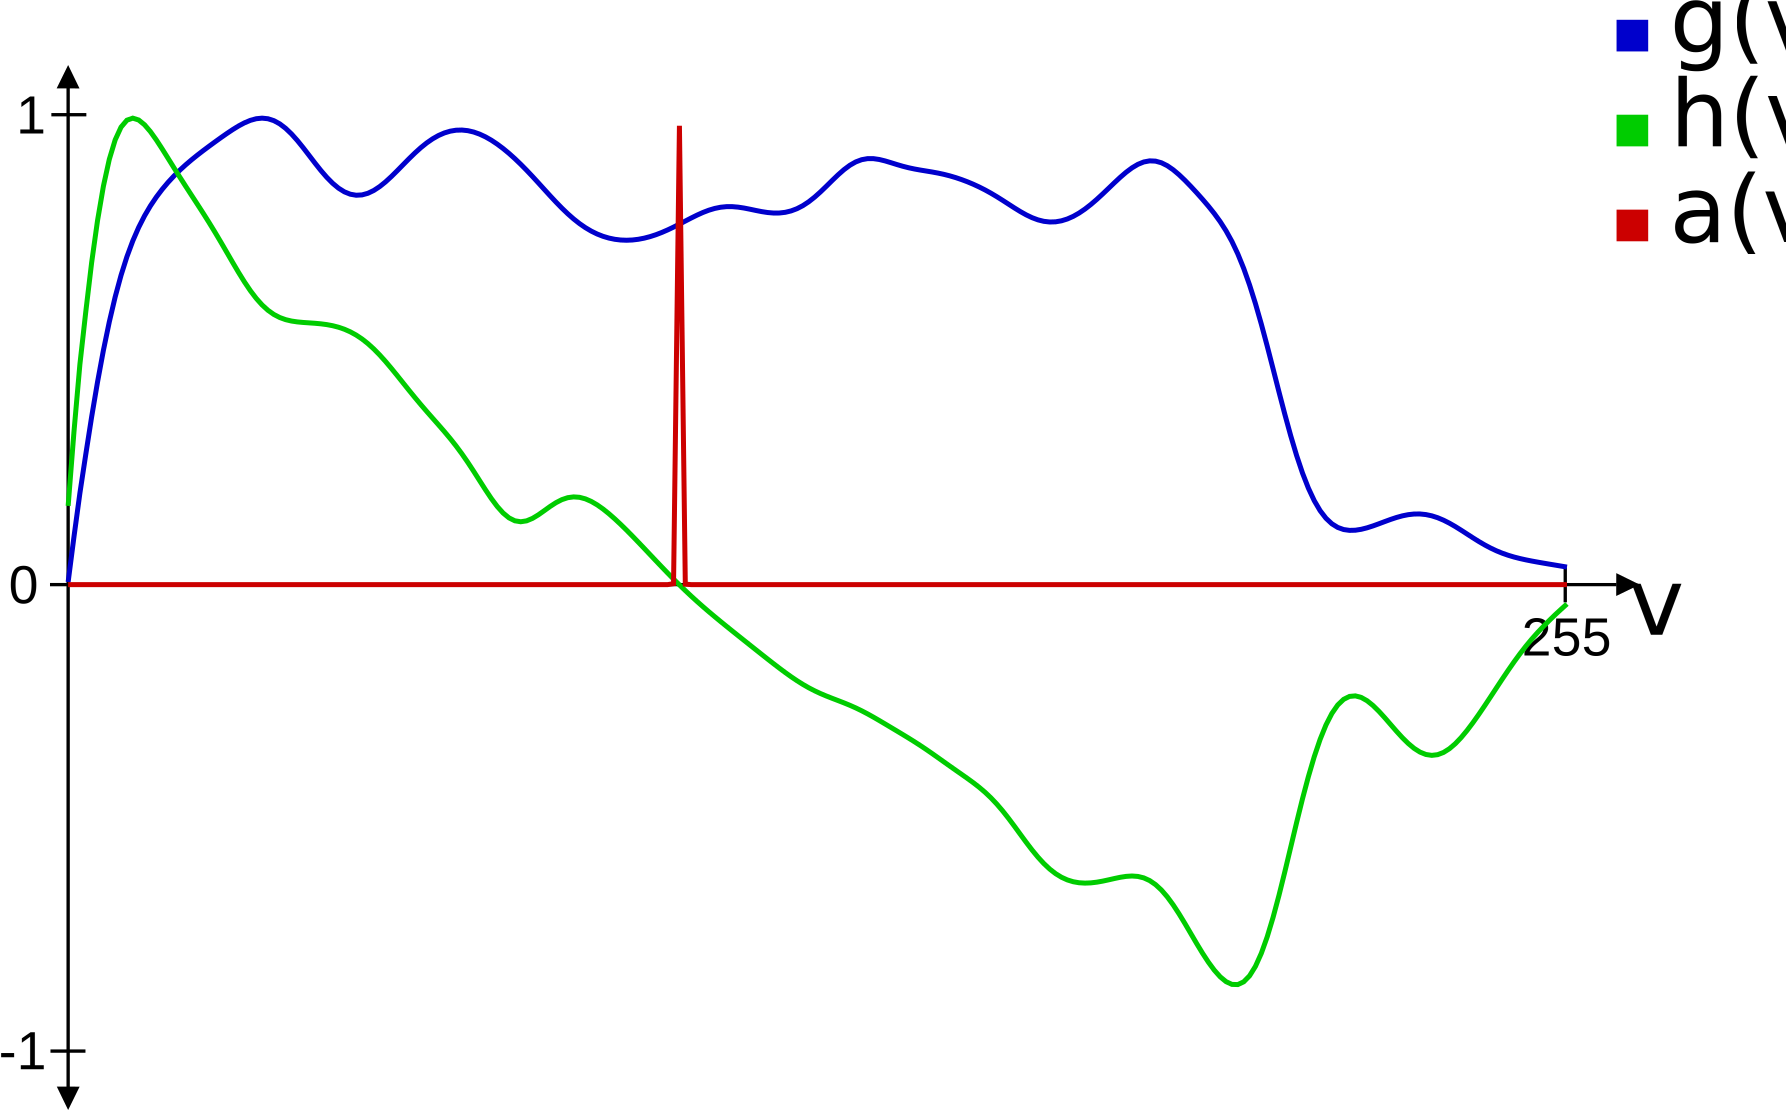
\includegraphics[width=0.7\textwidth]{images/r_box_sg_kd_ft}
		\label{fig:r_box_sg_kd_ft}
	}
	\subfigure[Visualização pela FT do método de \textit{Kindlmann e Durkin}.]
	{
		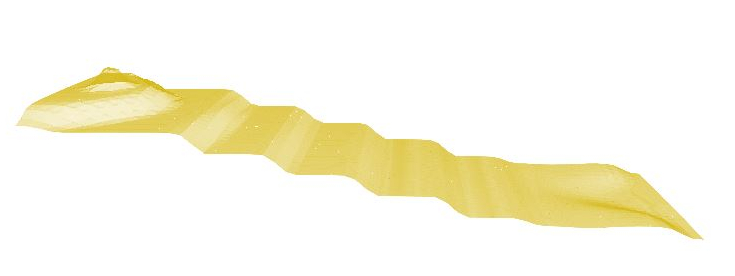
\includegraphics[width=0.7\textwidth]{images/r_box_sg_kd}
		\label{fig:r_box_sg_kd}
	}
	\subfigure[Função de transferência pelo método proposto.]
	{
		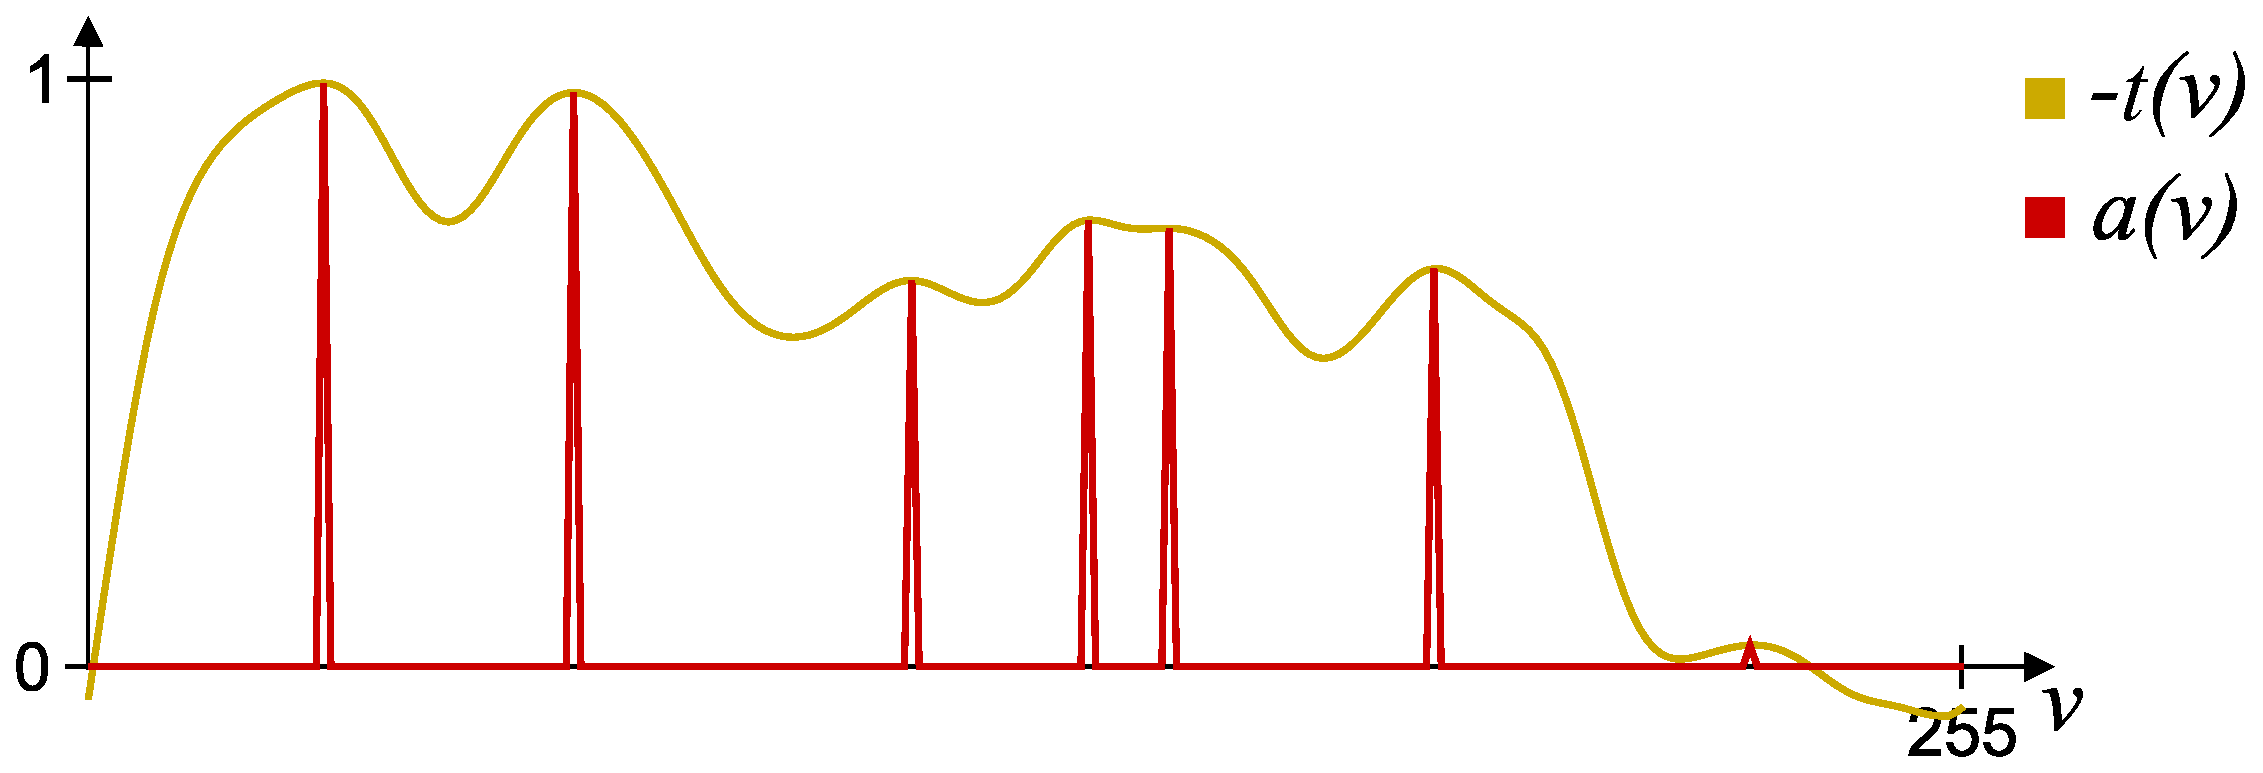
\includegraphics[width=0.7\textwidth]{images/r_box_sg_mine_ft}			\label{fig:r_box_sg_mine_ft}
	}
	\subfigure[Visualização pela FT do método proposto.]
	{
		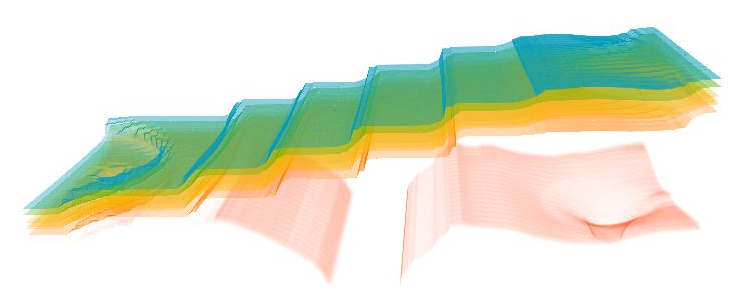
\includegraphics[width=0.7\textwidth]{images/r_box_sg_mine}	\label{fig:r_box_sg_mine}
	}
	\caption{Visualização e função de transferência do volume \quote{Caixa de sapato} com a propriedade saturação de gás.}
	\label{fig:r_box_sg}
\end{figure}

Texto...

%%%%%%%%%%%%%%%%%%%%%%%%%%%%%%%%%% BOX SW %%%%%%%%%%%%%%%%%%%%%%%%%%%%%%%%%%%%%
\begin{figure}[h]
	\centering
	\frame{
\includegraphics[width=0.5\textwidth]{images/r_box_sw_slice}}
	\caption{Fatia do volume \quote{Caixa de sapato} com a propriedade saturação de água.}
\end{figure}

\begin{figure}[h]
	\centering
	\subfigure[Função de transferência pelo método de \textit{Kindlmann e Durkin}.]
	{
		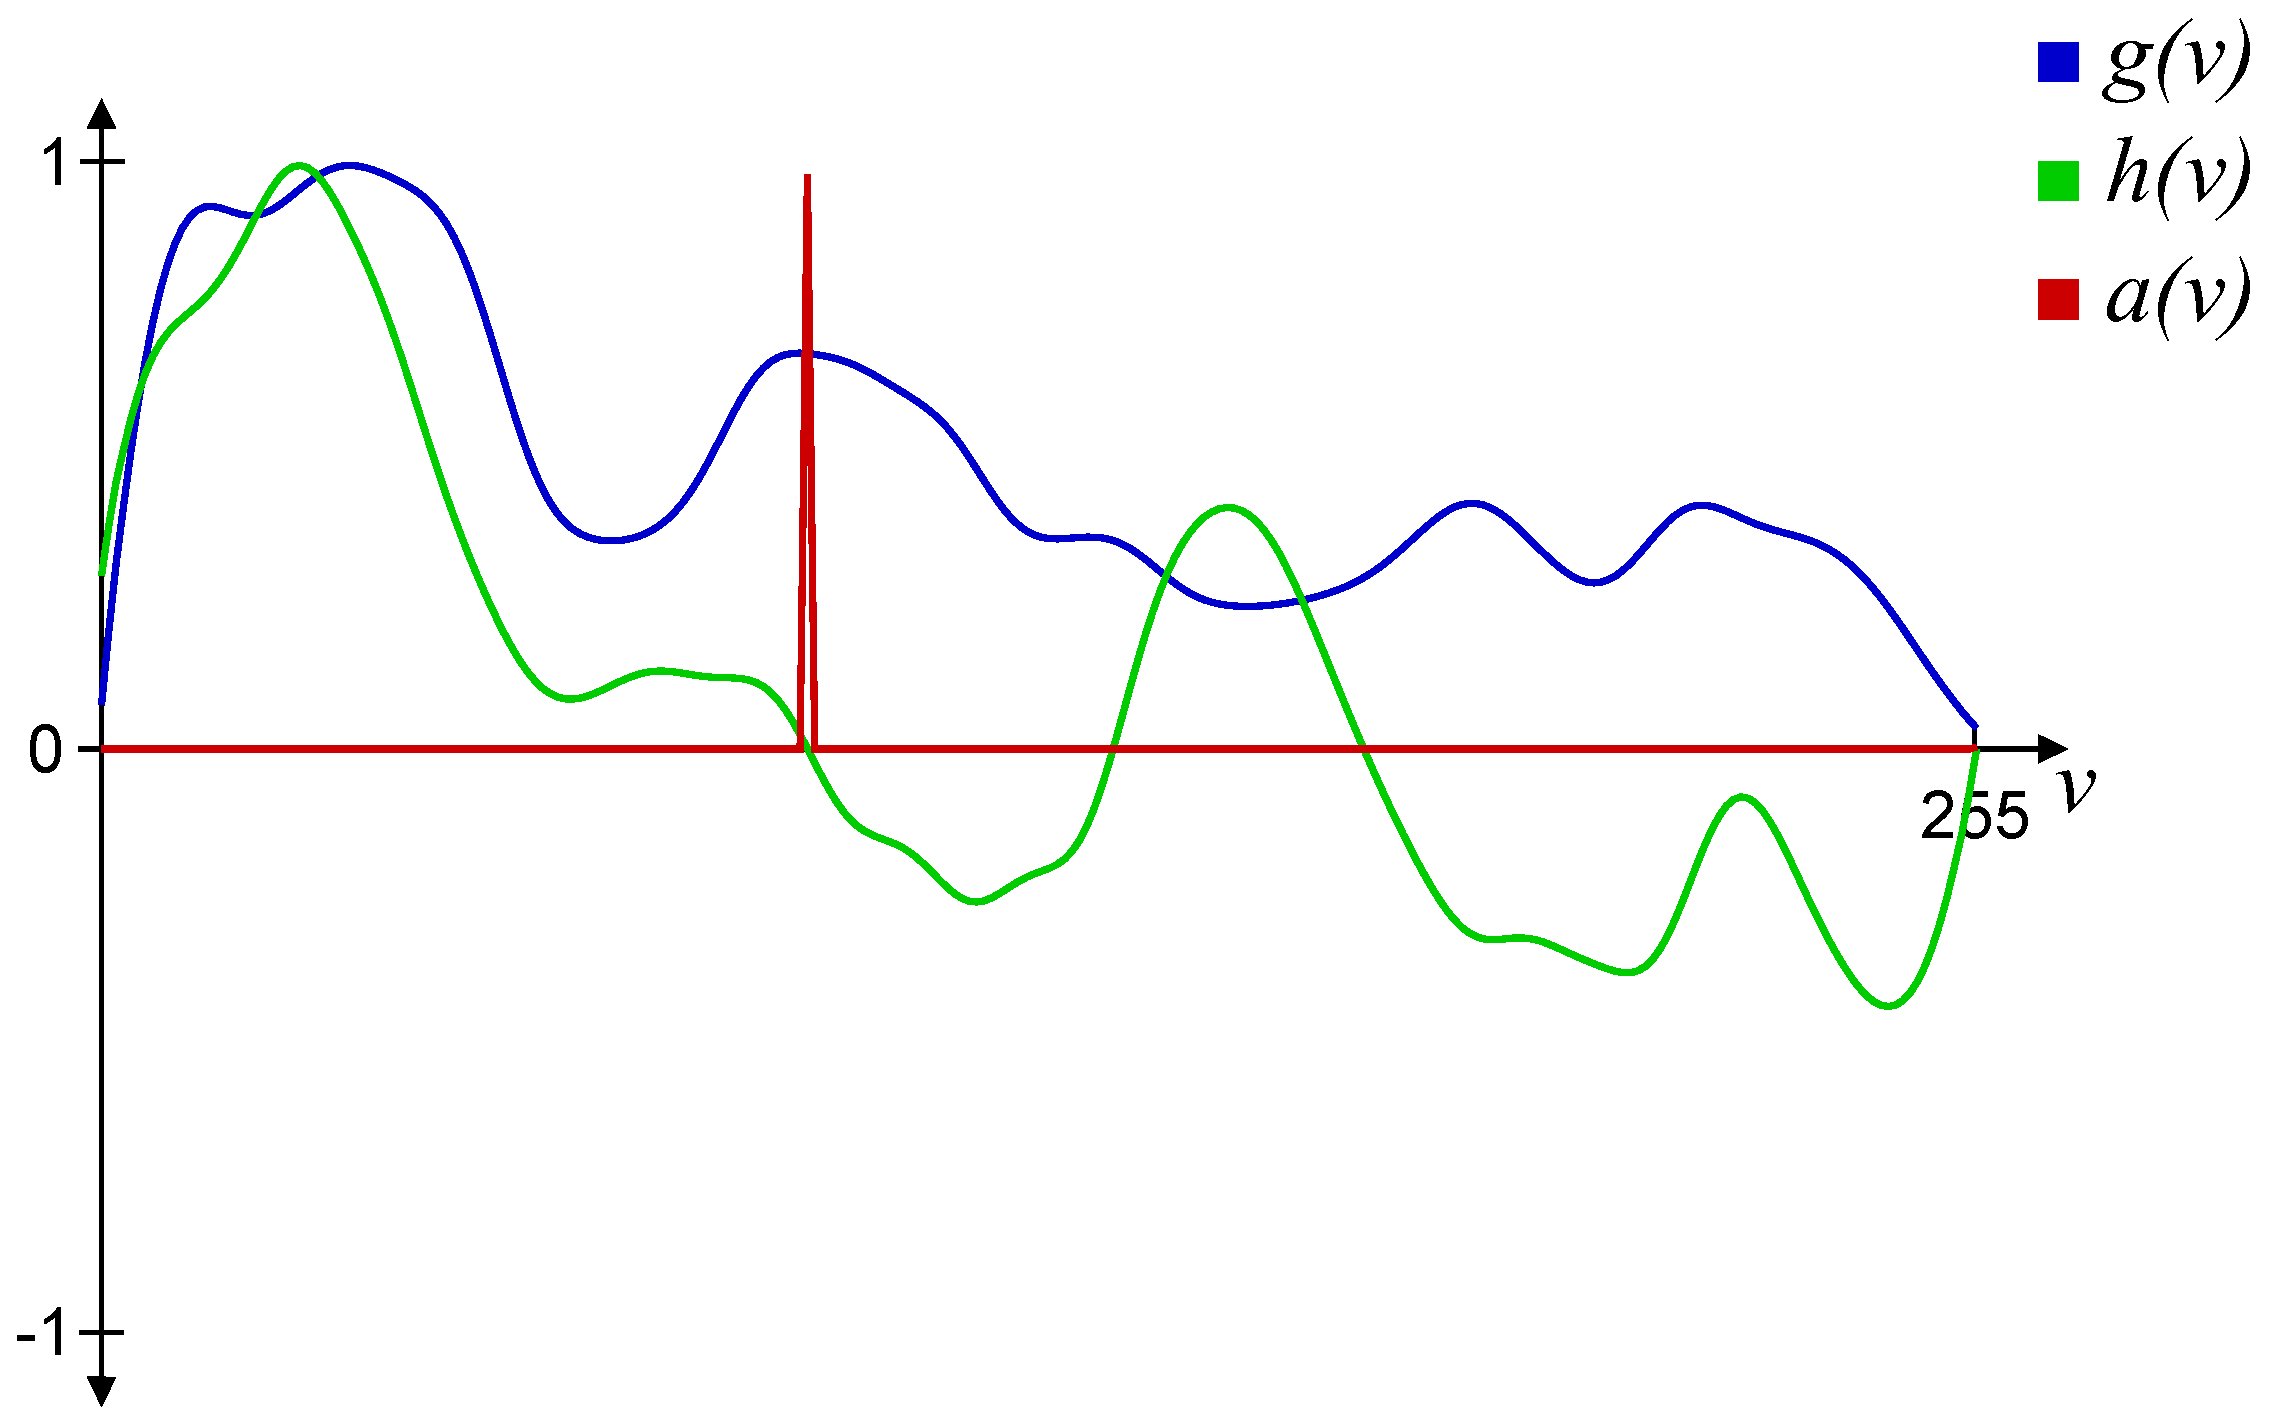
\includegraphics[width=0.7\textwidth]{images/r_box_sw_kd_ft}
		\label{fig:r_box_sw_kd_ft}
	}
	\subfigure[Visualização pela FT do método de \textit{Kindlmann e Durkin}.]
	{
		\includegraphics[width=0.7\textwidth]{images/r_box_sw_kd}
		\label{fig:r_box_sw_kd}
	}
	\subfigure[Função de transferência pelo método proposto.]
	{
		\includegraphics[width=0.7\textwidth]{images/r_box_sw_mine_ft}			\label{fig:r_box_sw_mine_ft}
	}
	\subfigure[Visualização pela FT do método proposto.]
	{
		\includegraphics[width=0.7\textwidth]{images/r_box_sw_mine}	\label{fig:r_box_sw_mine}
	}
	\caption{Visualização e função de transferência do volume \quote{Caixa de sapato} com a propriedade saturação de água.}
	\label{fig:r_box_sw}
\end{figure}

Texto...

%%%%%%%%%%%%%%%%%%%%%%%%%%%%%%%%%% Pituba %%%%%%%%%%%%%%%%%%%%%%%%%%%%%%%%%%%%%
\begin{figure}[h]
	\centering
	\includegraphics[width=0.7\textwidth]{images/pituba}
	\caption{...}
\end{figure}

Texto...